%%%%%%%%%%%%%%%%%%%%%%%%%%%%%%%%%%%%%%%%%
% The Legrand Orange Book
% LaTeX Template
% Version 3.1 (February 18, 2022)
%
% This template originates from:
% https://www.LaTeXTemplates.com
%
% Authors:
% Vel (vel@latextemplates.com)
% Mathias Legrand (legrand.mathias@gmail.com)
%
% License:
% CC BY-NC-SA 4.0 (https://creativecommons.org/licenses/by-nc-sa/4.0/)
%
% Compiling this template:
% This template uses biber for its bibliography and makeindex for its index.
% When you first open the template, compile it from the command line with the 
% commands below to make sure your LaTeX distribution is configured correctly:
%
% 1) pdflatex main
% 2) makeindex main.idx -s indexstyle.ist
% 3) biber main
% 4) pdflatex main x 2
%
% After this, when you wish to update the bibliography/index use the appropriate
% command above and make sure to compile with pdflatex several times 
% afterwards to propagate your changes to the document.
%
%%%%%%%%%%%%%%%%%%%%%%%%%%%%%%%%%%%%%%%%%

%----------------------------------------------------------------------------------------
%	PACKAGES AND OTHER DOCUMENT CONFIGURATIONS
%----------------------------------------------------------------------------------------

\documentclass[
	11pt, % Default font size, select one of 10pt, 11pt or 12pt
	fleqn, % Left align equations
	a4paper, % Paper size, use either 'a4paper' for A4 size or 'letterpaper' for US letter size
	%oneside, % Uncomment for oneside mode, this doesn't start new chapters and parts on odd pages (adding an empty page if required), this mode is more suitable if the book is to be read on a screen instead of printed
]{LegrandOrangeBook}

% Book information for PDF metadata, remove/comment this block if not required 


\addbibresource{sample.bib} % Bibliography file

\definecolor{ocre}{RGB}{243, 102, 25} % Define the color used for highlighting throughout the book

\chapterimage{orange2.jpg} % Chapter heading image
\chapterspaceabove{6.5cm} % Default whitespace from the top of the page to the chapter title on chapter pages
\chapterspacebelow{6.75cm} % Default amount of vertical whitespace from the top margin to the start of the text on chapter pages

%----------------------------------------------------------------------------------------

\begin{document}




%----------------------------------------------------------------------------------------
%	TITLE PAGE
%----------------------------------------------------------------------------------------

\titlepage % Output the title page
	{
\includegraphics[width=\paperwidth]{Images/background.pdf}} % Code to output the background image, which should be the same dimensions as the paper to fill the page entirely; leave empty for no background image
	{ % Title(s) and author(s)
		\centering\sffamily % Font styling
		{\Huge\bfseries TS CPRP 1 \\ Sciences de l'ingénieur\par} % Book title
		\vspace{16pt} % Vertical whitespace
		{\LARGE Séquence 1 : Communiquer dans l'industrie\par} % Subtitle
		\vspace{24pt} % Vertical whitespace
		{\huge\bfseries \par} % Author name
	}









%----------------------------------------------------------------------------------------
%	SECTIONING EXAMPLES CHAPTER
%----------------------------------------------------------------------------------------


\part{Communiquer dans l'industrie}

%----------------------------------------------------------------------------------------
%	MATHEMATICS EXAMPLES CHAPTER
%----------------------------------------------------------------------------------------

\chapter{Représentation normée des systèmes}

\section{Introduction}


S’échanger des \textbf{informations} est essentiel pour construire le monde d’aujourd’hui. Les exigences que nous avons, vis-à-vis des \textbf{risques} (la musique d'un airpod de doit pas dépasser 100 dB), du \textbf{confort} (la température de la salle de classe ne doit pas être inférieure à 16$^{\circ}$), de l'\textbf{accessibilités} (l'espacement entre les allées doivent permettre le passage d'une chaise roulante) ou des \textbf{performances} (le véhicule doit avoir une puissance max de 100 chevaux) des systèmes que nous concevons doivent être comprise de toute.s. Cet objectif impose d’être rigoureux pour éviter les mésententes. Le temps et le coût étant pris en compte, nous voulons éviter les hors-sujets une fois le travail déjà terminé. Nous essayerons de traduire nos systèmes dans des langages ou des \textbf{schémas} compréhensible de l’industrie. Comme la grammaire en français nous impose des règles, la représentation des systèmes impose des \textbf{normes}, admises par la plupart du parc industriel mondial.\\


Il existe trois types de normes :
\begin{enumerate}
    \item obligatoire / réglementaire ;
    \item volontaire / certifiable ;
    \item non certifiable.
\end{enumerate}


\begin{figure}[H] % Use [H] to suppress floating and place the figure/table exactly where it is specified in the text
	\centering % Horizontally center the figure on the page
	
\includegraphics[width=0.7\textwidth]{Images/Logo1.JPG} % Include the figure image
	\caption{Logo de différents organismes de normalisation.}
	\label{logo} % Unique label used for referencing the figure in-text
\end{figure}



\section{Système de normalisation}

\begin{corollary}[S2.4] 
Représentations graphiques dérivées des maquettes numériques \\
\textbf{C2.3} Synthétiser une information \\
\textbf{C5.3} \& \textbf{C6.1} Formuler, décoder et synthétiser un cahier des charges fonctionnel ou un dossier de conception \\
Langage de description SysML : \textbf{S1.1.1}


\end{corollary}

\begin{definition}{Normes}\index{Norme}

    La normalisation a pour objet de fournir des documents de référence portant sur des règles, des caractéristiques, des recommandations ou des exemples de bonnes pratiques, relatives à des produits, à des services, à des méthodes, à des processus ou à des organisations.\\ \textit{https://www.entreprises.gouv.fr/}
\end{definition}


En France, inventer et modifier les normes, c'est la mission de l’Association française de normalisation (AFNOR) c'est "notre" organisme national de normalisation (ONN).  Elle utilise ses normes comme support de la réglementation (obligatoire ou non). Quand une norme \textbf{rentre en application} elle peut être destinée à notre pays, l'Europe ou pour l'international.

\begin{theorem}
    Le nom des différentes normes ou organisme de norme (obligatoire ou non) sont :
    \begin{itemize}
    \item AFNOR - Association française de normalisation (elle édite les normes "NF");
        \item NF - Norme Française ;
        \item ISO - International organization for standartization (c'est une fédération mondiale d'autre d'organismes nationaux de normalisation. On les appelles "membres de l'ISO");
        \item EN - Normes européennes ;
        \item DIN - Institut allemand de normalisation;
        \item ANSI -  Institut national de normalisation américain.
    \end{itemize}
\end{theorem}

\begin{remark}
Notez qu'une entreprise se situant en France peut se certifier avec une norme Américaine. Si elle travail avec des français cela n'a pas grand intérêt, mais si elle traite exclusivement en Amérique c'est possible.
\end{remark}


\begin{figure}[H] % Use [H] to suppress floating and place the figure/table exactly where it is specified in the text
	\centering % Horizontally center the figure on the page
	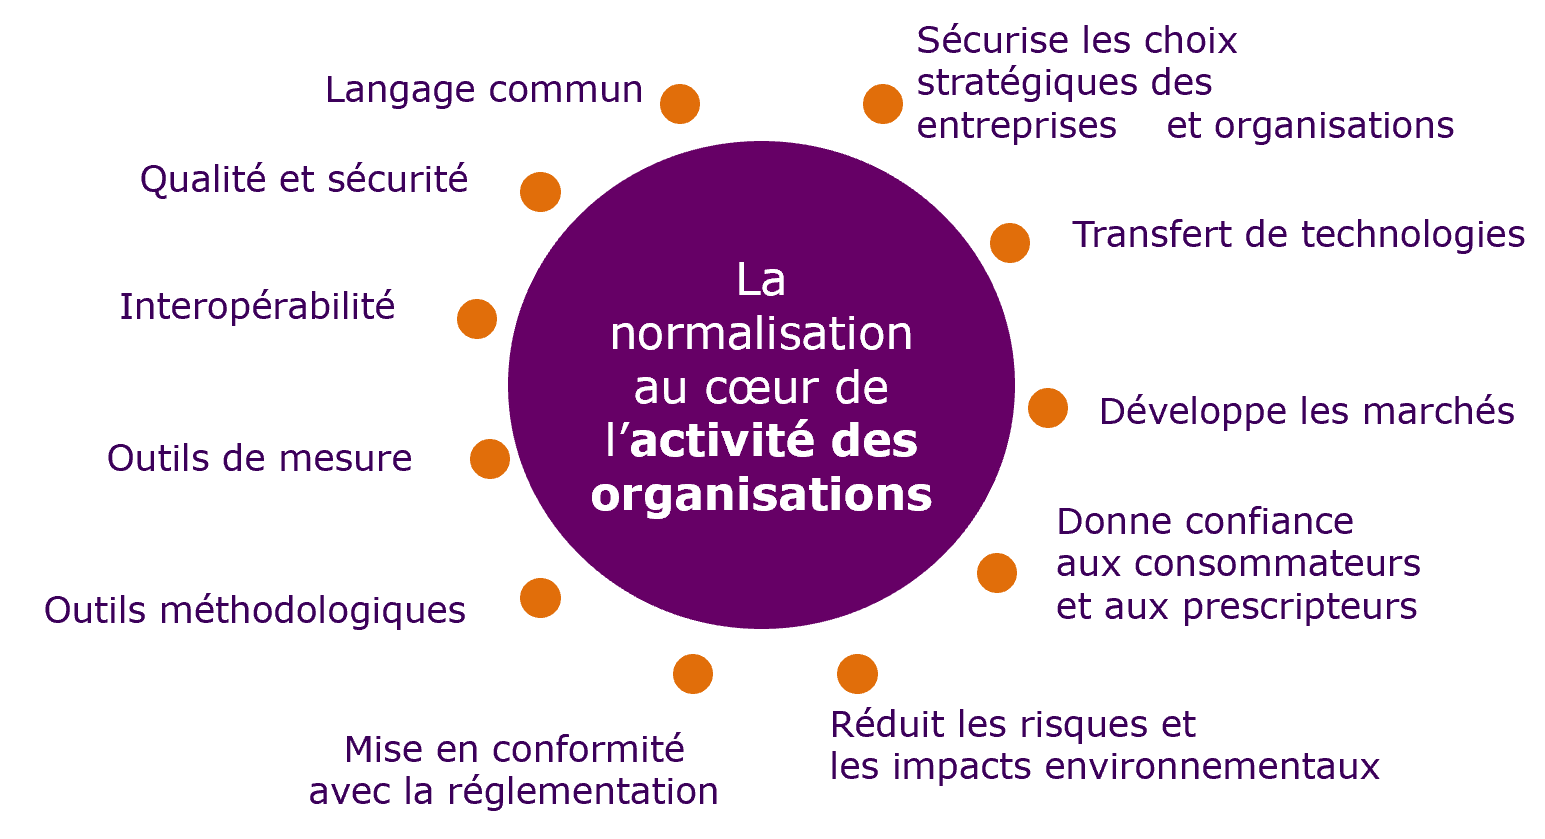
\includegraphics[width=0.7\textwidth]{AFNOR.PNG} % Include the figure image
	\caption{AFNOR Nomarlisation}
	\label{AFNOR} % Unique label used for referencing the figure in-text
\end{figure}



\section{Norme ISO 9001}\index{ISO 9001}


C’est une des normes les plus connues de l’industrie. Elle porte un regard général sur le management de la qualité. Elle apporte des garanties en termes de qualité organisationnelle au sein de tout type de structure. La certification ISO 9001 consiste à apporter la preuve qu'un système d'amélioration continue\footnote{Le Kaizen (en japonais), ou amélioration continue est né au Japon, peu après la fin de la Seconde Guerre mondiale. Il a gagné en popularité dans l’industrie et est devenu l’un des fondements de l’essor de Toyota, du petit fabricant automobile à l’un des plus grands constructeurs automobiles de la planète.} a été mis en place au sein de l'entreprise.\\

La norme ISO 9001 fait partie des normes qui tendent à améliorer la qualité, la sécurité et l'environnement de la planète (ou en tout cas, à ne pas empirer l'emprunte carbone humaine). Elle fait partie des normes que l'on doit obtenir si l'on veut avoir la certification \textbf{Qualité-Sécurité-Environnement}. La norme ISO 9001 (relative à la qualité) complète les normes ISO 45001 (pour la sécurité) et ISO 14001 (pour l’environnement) et permet aux entreprises d’avoir une politique globale de management des risques. La certification \textbf{QSE} (Figure \ref{logo_QSE}) est un acte volontaire et s’inscrit dans une démarche de progrès global à tous les niveaux de l’entreprise.



\begin{figure}[H] % Use [H] to suppress floating and place the figure/table exactly where it is specified in the text
	\centering % Horizontally center the figure on the page
	
\includegraphics[width=0.3\textwidth]{Images/Logo_QSE.png} % Include the figure image
	\caption{Logo de la certification QSE}
	\label{logo_QSE} % Unique label used for referencing the figure in-text
\end{figure}




\section{Norme NF Z68-020 ou NF ISO 841}\index{NF Z68-020}
Ce sont les normes qui précisent comment nous devons nommer les différents axes des machines outils. Bien que plus ancienne, vous verrez la plupart du temps la norme Z68-020. Cependant en Europe, cette norme a été remplacer. La norme actuellement en vigueur est la NF ISO 841 depuis septembre 2004.
\begin{definition}
La norme \textbf{NF Z68-020} [année 1968] définit la nomenclature des \textbf{axes et des mouvements} pour la commande numérique des machines.\footnote{https://www.boutique.afnor.org/}
\end{definition}


\begin{definition}
   La norme \textbf{NF ISO 841} [année 2004] définit les systèmes d'automatisation industrielle (Commande numérique des machines), les\textbf{ systèmes de coordonnées} des MOCN et la nomenclature de leurs \textbf{mouvements}\footnote{https://www.boutique.afnor.org/}.
\end{definition}




Les éléments de cette normes sont au coeur de la compréhension des dessins des pièces que l'on souhaite réaliser. Le but n'est pas de les apprendre d'un coup par coeur. Au cours des deux années de BTS ces définitions seront connues par l'habitude des les côtoyer.\\



\begin{definition}[Axes]\index{Axes}
    On dira qu'un machine possède " un axe " si le mouvement est continuellement commandé numériquement en \textbf{vitesse} et en \textbf{position}. Si l'axe est seulement commandé en vitesse ou l'inverse, on l'appellera "demi-axe".
\end{definition}


\begin{figure}[h] % Use [H] to suppress floating and place the figure/table exactly where it is specified in the text
	\centering % Horizontally center the figure on the page
	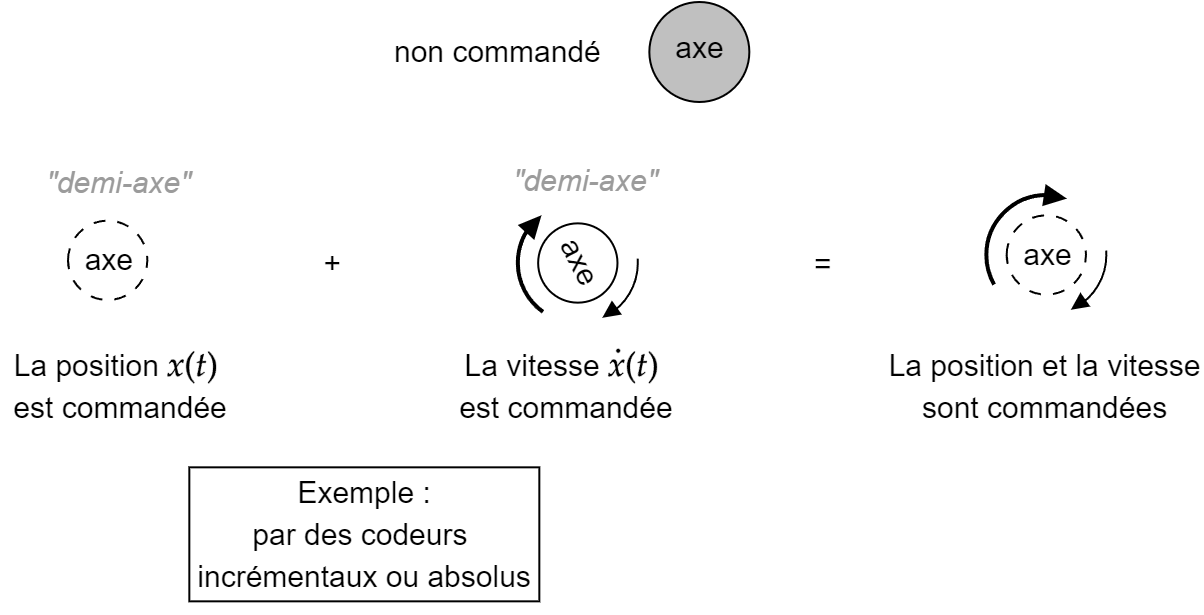
\includegraphics[width=1\textwidth]{Images/C1.png} % Include the figure image
	\caption{Schéma de commande des axes MOCN.}
	\label{logo_C1} % Unique label used for referencing the figure in-text
\end{figure}


\begin{definition}[L'axe $\overrightarrow{Z}$]\index{Axe Z}
    Il est situé parallèlement à l’axe de la broche principale quelle que soit la machine ou perpendiculaire à la table pour les machines qui ne possèdent pas de broche.
\end{definition}

\begin{definition}[L'axe $\overrightarrow{X}$]\index{Axe X}
    Il est associé au mouvement qui défini le plus grand déplacement après avoir situé l’axe Z. 
\end{definition}

\begin{definition}[L'axe $\overrightarrow{Y}$]\index{Axe Y}
    Il forme avec les axes X et Z un trièdre de sens direct. Le sens positif (+) d’un mouvement de chariot provoque l’éloignement de l’outil par rapport à la pièce considérée comme fixe. 
\end{definition}


\begin{figure}[H] % Use [H] to suppress floating and place the figure/table exactly where it is specified in the text
	\centering % Horizontally center the figure on the page
	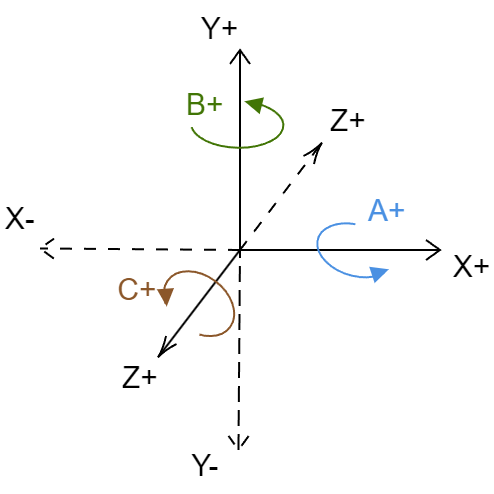
\includegraphics[width=0.6\textwidth]{Images/axe1.png} % Include the figure image
	\caption{Le système de cordonnées (X, Y, Z) est un système cartésien de sens direct lié à une pièce placée sur la machine. Exemple : Sur une MOCN, on peut mettre manuellement en rotation la broche dans le sens direct en appuyant sur le bouton \textbf{C+} du pupitre de commande.}
	\label{Axes_1} % Unique label used for referencing the figure in-text
\end{figure}


\begin{figure}[H] % Use [H] to suppress floating and place the figure/table exactly where it is specified in the text
	\centering % Horizontally center the figure on the page
	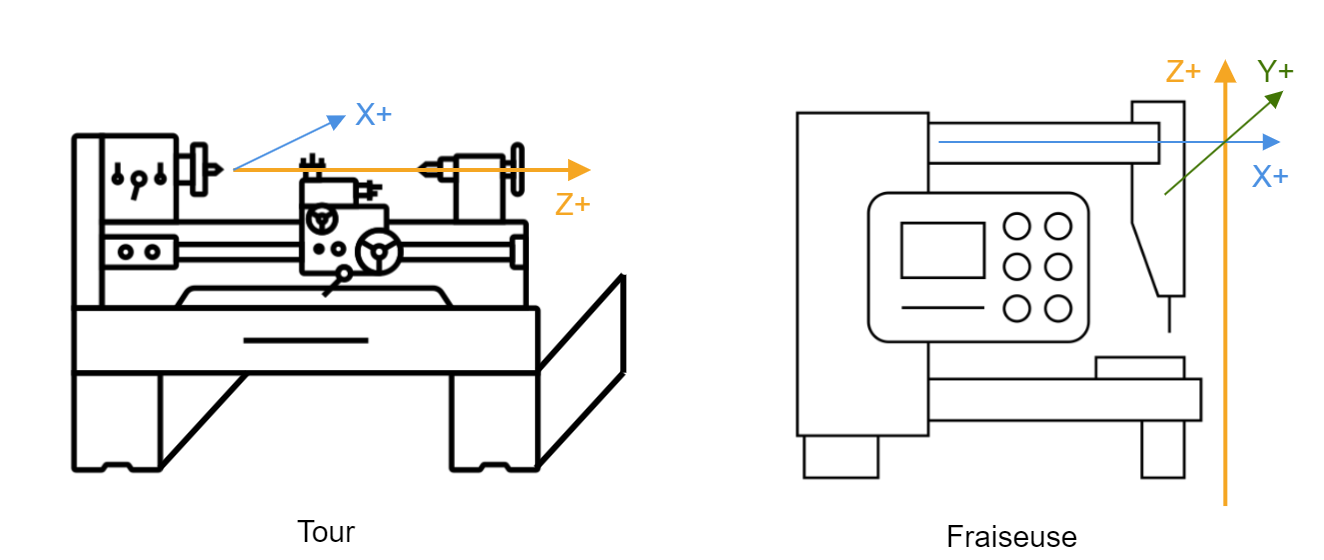
\includegraphics[width=1.1\textwidth]{Images/axe2.png} % Include the figure image
	\caption{Pour les machines conventionnelles ou MOCN simple, les axes sont orientés comme ci-dessus. Le déplacement positif (+) doit éloigner l'outil de la pièce.}
	\label{Axes_2} % Unique label used for referencing the figure in-text
\end{figure}





\section*{Exercice}\index{Exercices. Trouver les axes d'une MOCN}
But : Indiquer ou sont les axes, leur nom et orientation et remplir le tableau.
\begin{figure}[H] % Use [H] to suppress floating and place the figure/table exactly where it is specified in the text
	\centering % Horizontally center the figure on the page
   \fbox{
	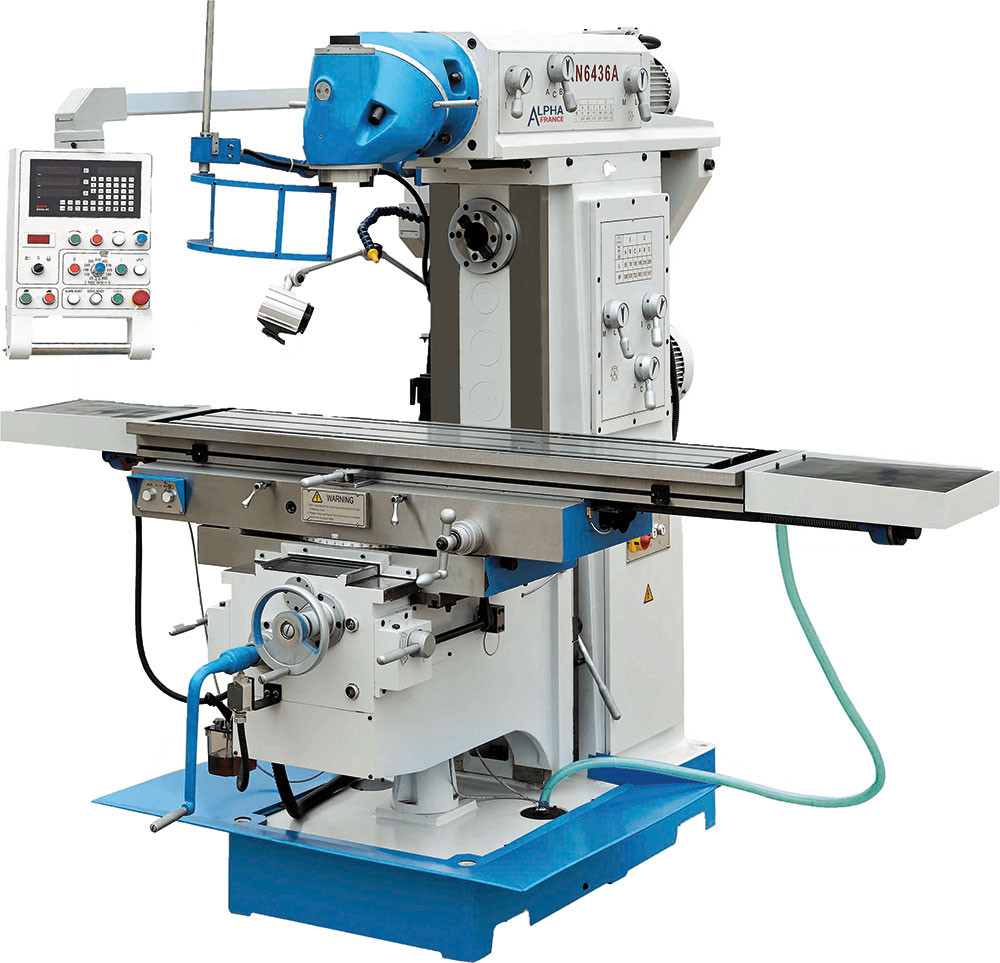
\includegraphics[width=0.9\textwidth]{Images/608.jpg} % Include the figure image
        }
	%\caption{Indiquez}
	\label{Exo_1} % Unique label used for referencing the figure in-text
\end{figure}


\begin{table}[H] % Use [H] to suppress floating and place the figure/table exactly where it is specified in the text
	\centering % Horizontally center the table on the page
	\begin{tabular}{L{0.15\textwidth} R{0.15\textwidth} R{0.15\textwidth}} % Specify column alignment with L{width}, C{width} and R{width} for fixed-width columns, or the default latex l, c and r for flexible-width columns
		\toprule
		\textbf{Type de MOCN} & \textbf{Nbr d'axe} & \textbf{Noms axes}\\
		\midrule
		  &  &  \\
		  &  &  \\
		  &  &  \\
		\bottomrule
	\end{tabular}
	%\caption{Table caption.}
	\label{Z12} % Unique label used for referencing the table in-text
\end{table}






But : Indiquer ou sont les axes, leur nom et orientation et remplir le tableau.
\begin{figure}[H] % Use [H] to suppress floating and place the figure/table exactly where it is specified in the text
	\centering % Horizontally center the figure on the page
   \fbox{
	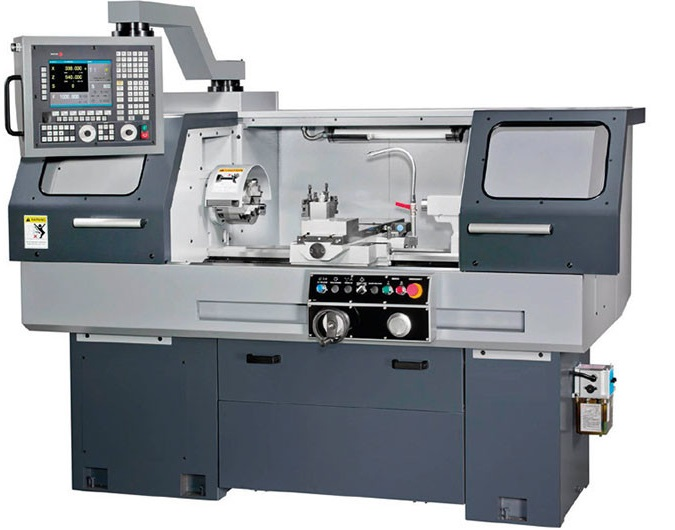
\includegraphics[width=0.9\textwidth]{Images/4959.jpg} % Include the figure image
        }
	%\caption{Indiquez}
	\label{Exo_2} % Unique label used for referencing the figure in-text
\end{figure}


\begin{table}[H] % Use [H] to suppress floating and place the figure/table exactly where it is specified in the text
	\centering % Horizontally center the table on the page
	\begin{tabular}{L{0.15\textwidth} R{0.15\textwidth} R{0.15\textwidth}} % Specify column alignment with L{width}, C{width} and R{width} for fixed-width columns, or the default latex l, c and r for flexible-width columns
		\toprule
		\textbf{Type de MOCN} & \textbf{Nbr d'axe} & \textbf{Noms axes}\\
		\midrule
		  &  &  \\
		  &  &  \\
		  &  &  \\
		\bottomrule
	\end{tabular}
	%\caption{Table caption.}
	\label{tab:example} % Unique label used for referencing the table in-text
\end{table}




\section{Norme ISO 2768}
\begin{definition}
    La norme vise à simplifier les dessins techniques. Elle indique les tolérances générales (pour les dimensions linéaires et angulaires), et les tolérances géométriques qui n'ont pas d'indication de tolérances sur le schéma. Selon la cotation du schéma, il y aura quatre classes de tolérance possible.\footnote{https://www.iso.org/} \\
\end{definition}


En	construction	mécanique,	la	tolérances	générales 2768	est	utilisée pour	:\\
\begin{itemize}
    \item éviter d'écrire un nombre trop important	d'indications sur le dessin ;
    \item avoir	une	pièce entièrement tolérancée.\\
\end{itemize}




Pour indiquer que nous utilisons cette norme nous devons :\\
\begin{enumerate}
    \item  Prendre une zone suffisamment près du	cartouche;
    \item Inscrire " \textbf{Tolérances générales} " 
    \item Inscrire \textbf{ISO	2768}	(numéro de la norme utilisée);
    \item la classe de précision :
          \begin{itemize} 
            \item f pour "fine" (fin);
            \item m pour "medium" (moyen);
            \item c pour "coarse" (grossière - large);
            \item v pour "very coarse" (très grossière - très large).
           \end{itemize}
        \item la classe	de	précision pour les	tolérances géométriques :
         \begin{itemize}           
                \item H pour fin;
                \item K pour moyen;
                \item M pour large.
            \end{itemize}
\end{enumerate}


\subsection*{Extrait Examen BTS CPRP 2020}

Prenons l'exemple du BTS 2020 Figure \ref{ABTS1}.\\ 
Certaines côtes ont des tolérances, comme ce diamètre :  \begin{tikzpicture}  {$ \varnothing 3^{ \begin{array}{l}
+0,20\\
-0
\end{array}}$}; \end{tikzpicture}  

\vspace{0.5 cm}

Ou la côte suivante : 
\begin{tikzpicture}  {$ 8,10^{ \begin{array}{l}
+0,10\\
0
\end{array}}$}; \end{tikzpicture} \\
D'autres ont seulement une côte, sans tolérances visible directement : 0,70 ou $\varnothing$2,50.\\
Pour les côtes qui n'ont pas de tolérances, comment savoir \textbf{la marge d'erreur acceptée} ?\\
Essayez, pour les deux cotations énoncées juste avant, d'indiquer la tolérance en vous aidant du détail de la norme 2768 en annexe et de la Figure \ref{Tol2}.


\begin{table}[H] % Use [H] to suppress floating and place the figure/table exactly where it is specified in the text
	\centering % Horizontally center the table on the page
	\begin{tabular}{L{0.15\textwidth} R{0.15\textwidth} R{0.15\textwidth}} % Specify column alignment with L{width}, C{width} and R{width} for fixed-width columns, or the default latex l, c and r for flexible-width columns
		\toprule
		\textbf{0,70} & \textbf{} & \textbf{$\varnothing$2,50}\\
		\midrule
		  &  &  \\
		  & Tolérance $\pm$ &  \\
		  &  &  \\
		\bottomrule
	\end{tabular}
	%\caption{Table caption.}
	\label{Tol} % Unique label used for referencing the table in-text
\end{table}



\begin{figure}[H] % Use [H] to suppress floating and place the figure/table exactly where it is specified in the text
	\centering % Horizontally center the figure on the page
   \fbox{
	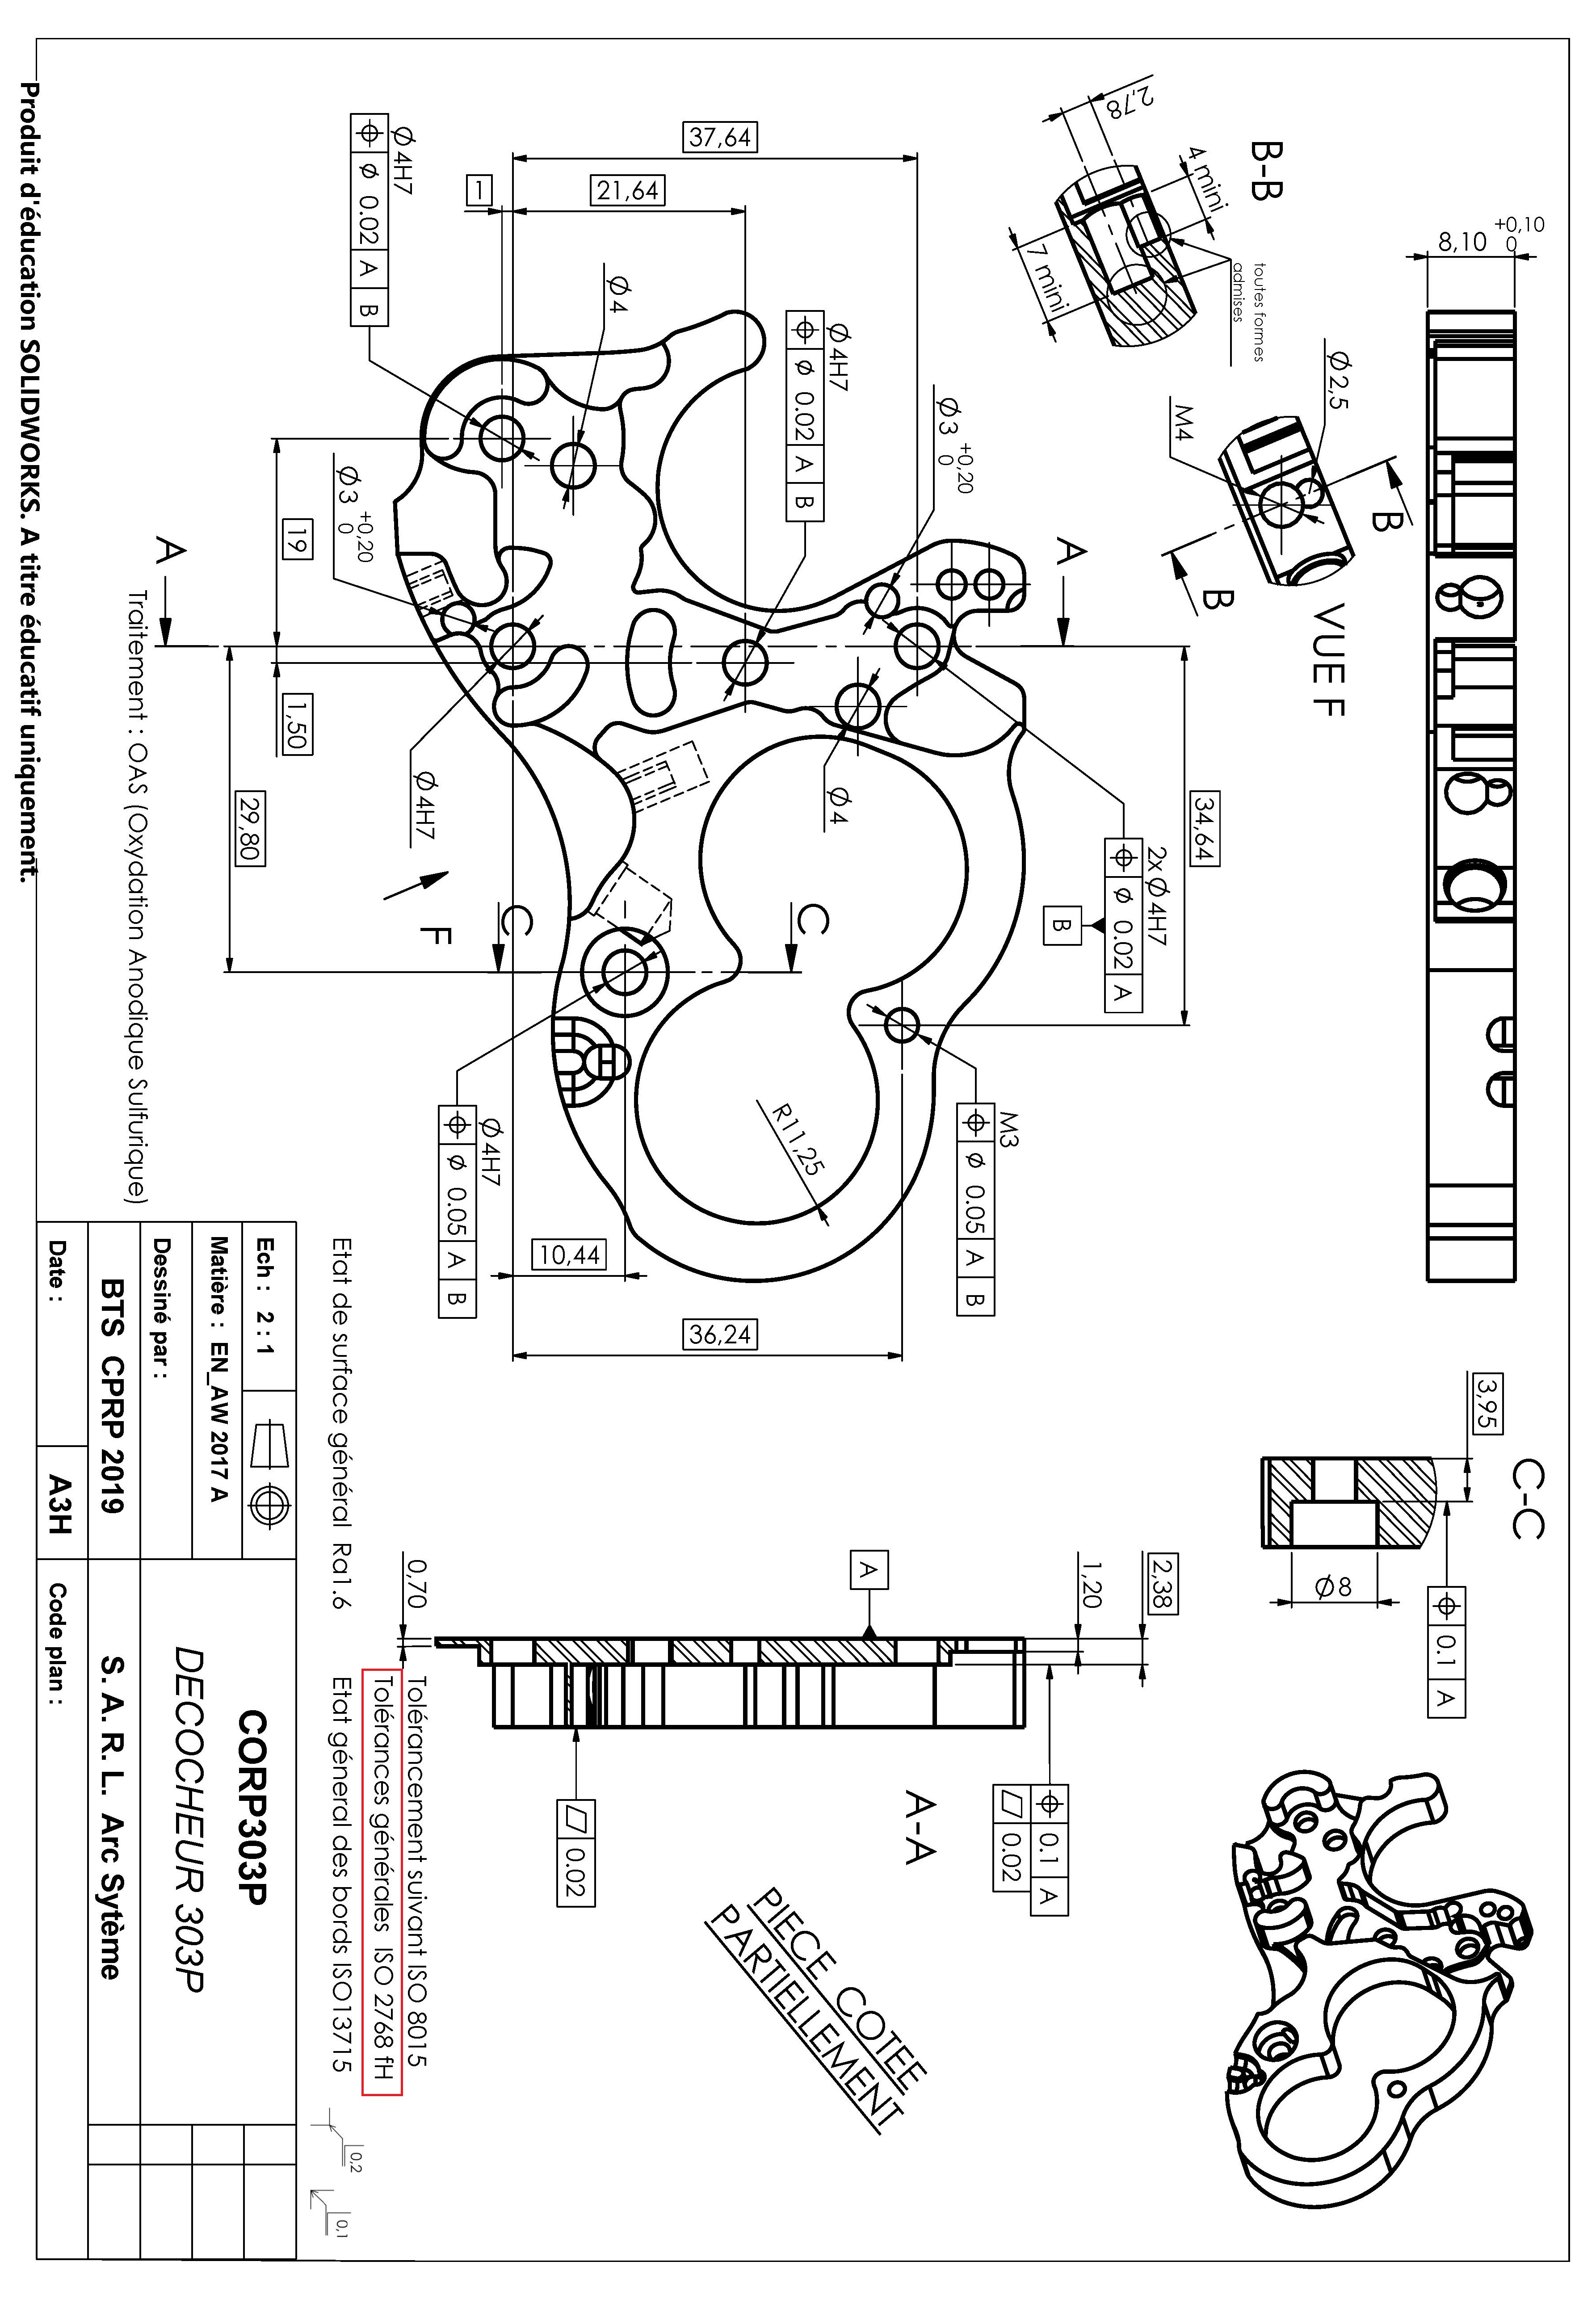
\includegraphics[width=0.9\textwidth]{Images/ABTS1.jpg} % Include the figure image
        }
	\caption{Modèle 303P de la société Arc Système. Il permet de tracter et de libérer la corde de manière reproductible en ayant pas (ou peu) d’influence sur sa trajectoire (ainsi que celle de la flèche). Il augmente considérablement la précision et la répétabilité du tir par rapport à un lâcher de corde manuel. Épreuve E4 : Conception préliminaire. Session 2020}
	\label{ABTS1} % Unique label used for referencing the figure in-text
\end{figure}

Pour résumer, la méthode peut être :\\
\begin{figure}[H] % Use [H] to suppress floating and place the figure/table exactly where it is specified in the text
	\centering % Horizontally center the figure on the page
   \fbox{
	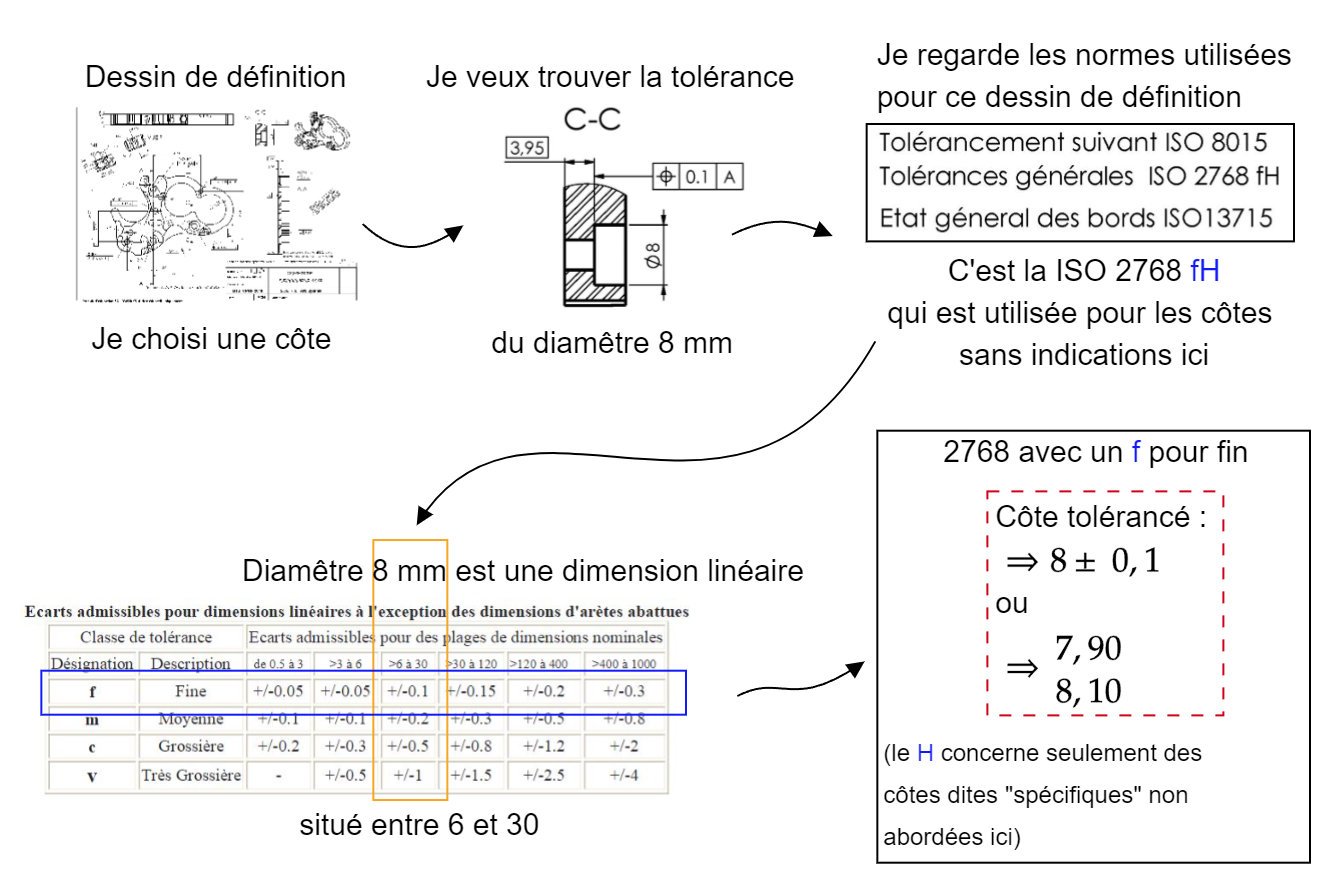
\includegraphics[width=1\textwidth]{Images/tol2.png} % Include the figure image
        }
	\caption{Méthode. Recherche des cotations générales.}\index{Méthode : Cotations générales}
	\label{Tol2} % Unique label used for referencing the figure in-text
\end{figure}









%----------------------------------------------------------------------------------------
%	PRESENTING INFORMATION/RESULTS EXAMPLES CHAPTER
%----------------------------------------------------------------------------------------

\chapterimage{Images/chapt2.jpg} % Chapter heading image
\chapterspaceabove{6.25cm} % Whitespace from the top of the page to the chapter title on chapter pages
\chapterspacebelow{7.5cm} % Amount of vertical whitespace from the top margin to the start of the text on chapter pages

\chapter{Représentation schématique}

%------------------------------------------------

\section{Langage SysML}

Souvent au début des sujets du BTS, le "\textbf{Systems Modeling Language}" est un incontournable de l'examen du brevet CPRP. Il décrit le système que vous allez étudier pendant 6 heures !\\
En fonction de ce qu'on souhaite décrire, on utilise un ou plusieurs des diagrammes répartis en 3 catégories (figure \ref{Sys1}).


\begin{figure}[H] % Use [H] to suppress floating and place the figure/table exactly where it is specified in the text
	\centering % Horizontally center the figure on the page
	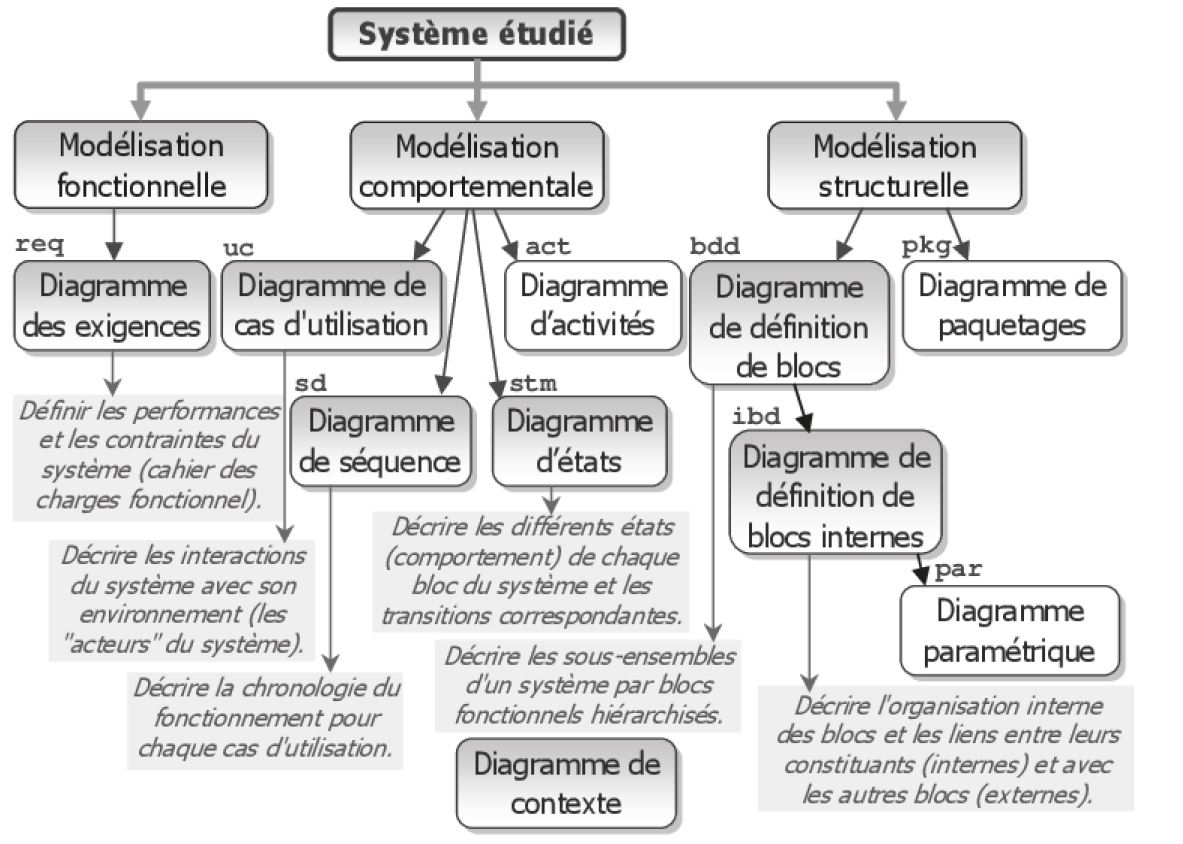
\includegraphics[width=1\textwidth]{Images/Sys1.JPG} % Include the figure image
	\caption{Model SysML}
	\label{Sys1} % Unique label used for referencing the figure in-text
\end{figure}



Chacune des trois catégories répond à une question :
\begin{itemize}
    \item modélisation fonctionnelle : « que doit faire le système ? »
    \item modélisation comportementale : « comment le système doit-il se comporter ? »
    \item modélisation structurelle : « comment le système est-il construit ? ».\\
\end{itemize}


Ces différentes modélisation permettent de situer la \textbf{frontière de l’étude} dans un contexte \textbf{pluri-technologique}. Le tout pour que le système réponde au Cahier des charges.\\

\begin{definition}[Cahier des charges (CdC)]\index{Cahier des charges}
    C’est un document par lequel le demandeur exprime son besoin (ou celui qu'il est chargé de
traduire) en terme de fonctions de services ou d’exigences. Pour chacune d’elles sont définis
des critères d’appréciation et leurs niveaux. Chacun de ces niveaux doit être assorti d’une
flexibilité (norme AFNOR X 50-150).\\
\end{definition}

\begin{figure}[H] % Use [H] to suppress floating and place the figure/table exactly where it is specified in the text
	\centering % Horizontally center the figure on the page
	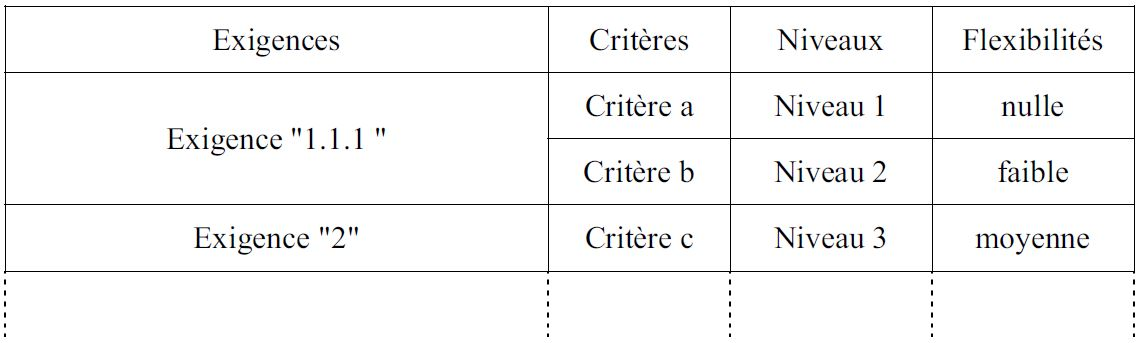
\includegraphics[width=1\textwidth]{Images/sys2.JPG} % Include the figure image
	\caption{Chaque exigence doit avoir un ou plusieurs critères, niveau et flexibilités.}
	\label{sys2} % Unique label used for referencing the figure in-text
\end{figure}

Les critères permettant d’apprécier un système sont notamment liés aux caractéristiques
techniques (tension d’alimentation, énergies, etc.), aux performances (force, vitesse, temps pour
passer de 0 à 100 km/h, etc.), à l’esthétique (notion très subjective), mais aussi à l’usage
(fiabilité, durée de vie, coût global de possession, etc.).
Le niveau permet de quantifier un critère en indiquant une valeur, un intervalle, une norme, etc.
La flexibilité donne une indication sur la marge de manœuvre laissée au concepteur.\\


Par exemple
\begin{itemize}
    \item Exigence : un aspirateur en fonctionnement ne doit pas déranger les autres occupants d'une habitation ;
    \item Critère : Bruit / Son ;
    \item Niveaux : Ne doit pas dépasser 80 dB ;
    \item Flexibilité : On autorise un dépassement de $5\%$.\\
\end{itemize}










\subsection{Exemple BTS 2020}

Le système suivant est celui de l'arc à poulie doté du système décocheur Arc Système 303P (figure \ref{fleche1}). 
\begin{figure}[H] % Use [H] to suppress floating and place the figure/table exactly where it is specified in the text
	\centering % Horizontally center the figure on the page
	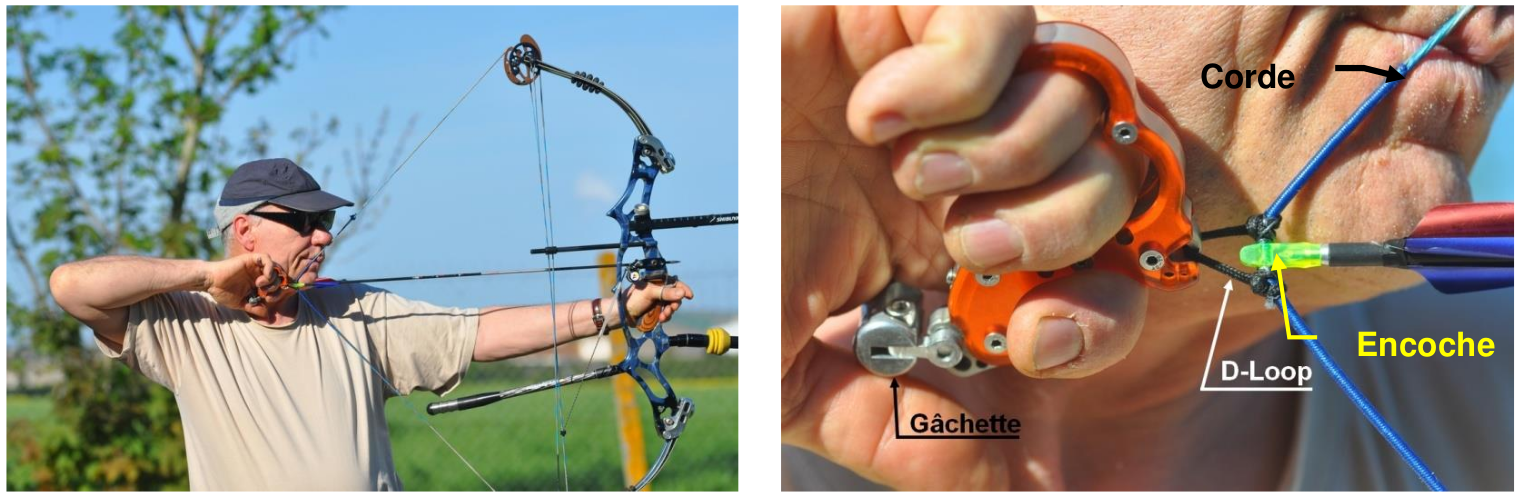
\includegraphics[width=0.7\textwidth]{Images/fleche1.png} % Include the figure image
	\caption{Système 303P}
	\label{fleche1} % Unique label used for referencing the figure in-text
\end{figure}
Dans les sciences de l'ingénieur, on s'intéresse aux écarts entre ce qu'on veut (en théorie), et se qui se passe vraiment (en pratique). On représente un schéma "fonctionnel" du système. Il permet de collecter et d'organiser toutes les exigences du système (caractéristiques ou performances théoriques attendues), sous forme textuelle. 

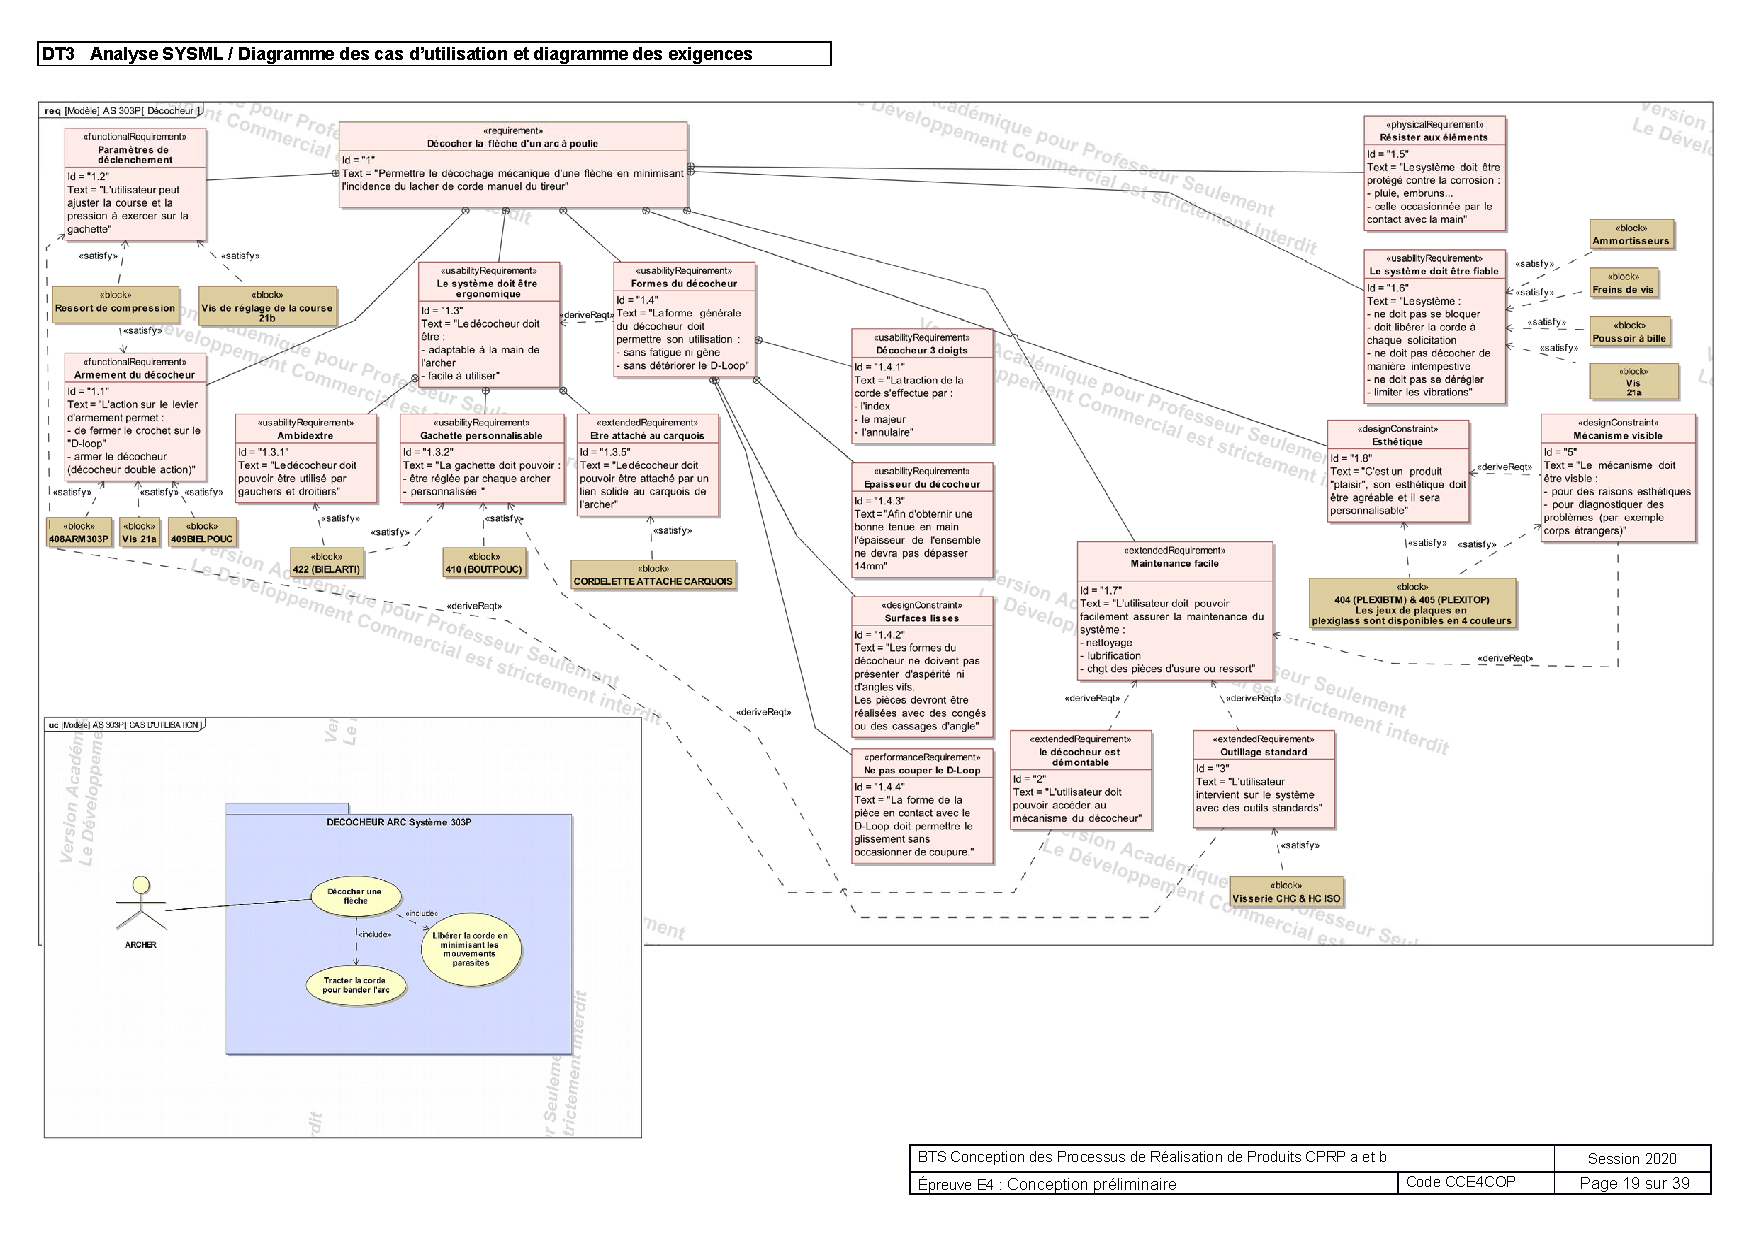
\includepdf[angle=90]{fleche2.pdf}

\begin{tcolorbox}[colback=gray!5!white,colframe=gray!75!ocre,title=Tiré du BTS 2020]\index{Exercice : SysML}
Adaptation ergonomique à l’archer : Id= "1.3". \\
\textbf{Question 1.2.1 }: Préciser quelles pièces permettent d’adapter le décocheur à la main de l’archer. \\


Réglage de la course de déclenchement : Id= "1.2"\\
\textbf{Question 1.2.2 }: Indiquer quelle pièce permet de régler la course de déclenchement.\\

\end{tcolorbox}



\begin{tcolorbox}[colback=gray!5!white,colframe=gray!75!gray,title=Réponses]


\vspace{8 cm}

\end{tcolorbox}




\section{Schéma bête à corne}
Les autres schémas très rependus dans les sujets sont les diagrammes de type "Bête à corne". Ils servirons aux candidat.e.s dans l'analyse/formulation du besoin. Il doit répondre essentiellement à trois questions :
\begin{enumerate}
    \item A qui rend-il service ?
    \item Sur quoi/qui agit-il ?
    \item Dans quel but ?\\
\end{enumerate}



Pour satisfaire le besoin auquel le produit répond, des Fonctions de Service, qui correspondent à des exigences, doivent être remplies par celui-ci : il faut les rechercher et dresser leur liste. Elles se répartissent en 2 catégories :

\begin{enumerate}
    \item Les Fonctions Principales (une ou plusieurs), FP1, FP2 etc. ce sont des Fonctions du produit correspondant aux raisons
pour lesquelles ce dernier a été créé : ce sont donc sa ou ses fonctions d’usage. On peut les déduire directement du
diagramme bête à corne ;
    \item les Fonctions Contraintes (une ou plusieurs), FC: le produit n’a pas été créé pour cela, mais le fait d’exister lui impose d’assurer certaines Fonctions, en relation avec d’autres éléments de son environnement (appelés EME, Eléments du Milieu Extérieur, ou Interacteurs) , autres que lui-même. Ce sont des Fonctions qui traduisent les contraintes liées à l’adaptation du produit à son environnement et à la prise en compte de ce dernier. Ce sont des obligations à satisfaire, dans différentes catégories.\\
\end{enumerate}


Les contraintes peuvent être classées en six
catégories :
\begin{itemize}
\item  Fonctionnelles : nécessaires pour remplir la FP
\item  Ergonomiques : faciliter l’utilisation
\item  Esthétiques : le rendre attrayant
\item  De sécurité : l’utiliser en toute sécurité-> normes
\item  Environnementales : être conçu et utilisé dans un
souci de développement durable
\item Economiques/commerciales : coût correspondant au
service, au budget, à la publicité.
\end{itemize}

Nous avons vu précédemment un système s'intégrant aux arcs dans le BTS 2020. Un diagramme bête à corne de ce système pourrait être le suivant.


\begin{figure}[H] % Use [H] to suppress floating and place the figure/table exactly where it is specified in the text
	\centering % Horizontally center the figure on the page
	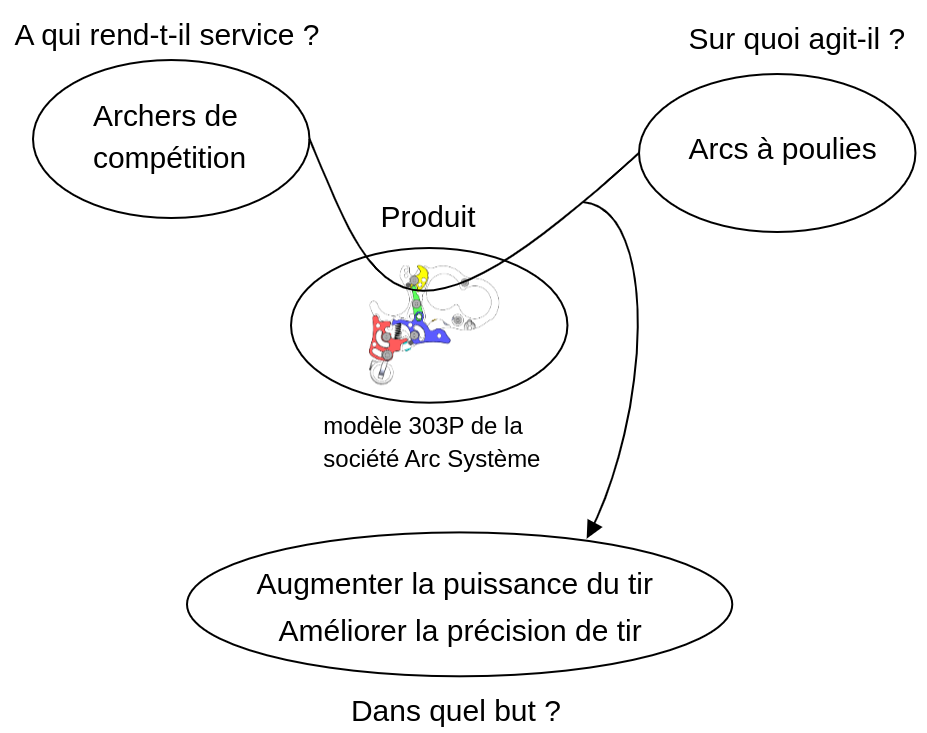
\includegraphics[width=0.7\textwidth]{Images/bete1.png} % Include the figure image
	\caption{Diagramme bête à corne du système 303p}
	\label{bete1} % Unique label used for referencing the figure in-text
\end{figure}

Toutes les fonctions,quelles soient \textbf{principales} ou de \textbf{contraintes}, peuvent ensuite être listées sous forme d'un tableau. Le diagramme bête à corne est donc une représentation claire et simplifiée du système.\\

Voici un autre exemple avec un stylo bille, avec le diagramme bête à corne et son tableau des fonctions associées.
\begin{figure}[H] % Use [H] to suppress floating and place the figure/table exactly where it is specified in the text
	\centering % Horizontally center the figure on the page
	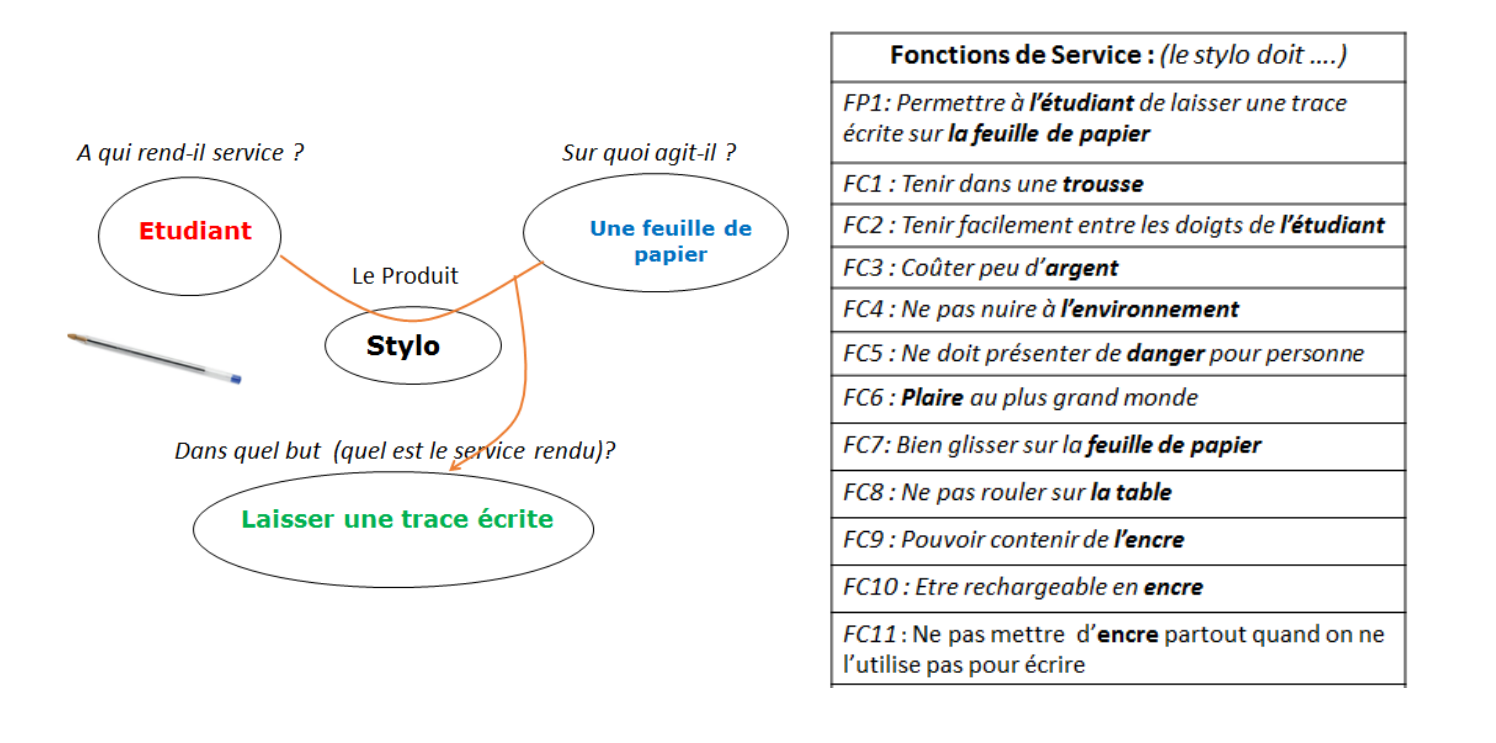
\includegraphics[width=1\textwidth]{Images/stylo3.png} % Include the figure image
	\caption{Diagramme bête à corne d'un stylo bille}
	\label{stylo} % Unique label used for referencing the figure in-text
\end{figure}



\subsection{Exemple BTS 2015}

\begin{figure}[H] % Use [H] to suppress floating and place the figure/table exactly where it is specified in the text
	\centering % Horizontally center the figure on the page
	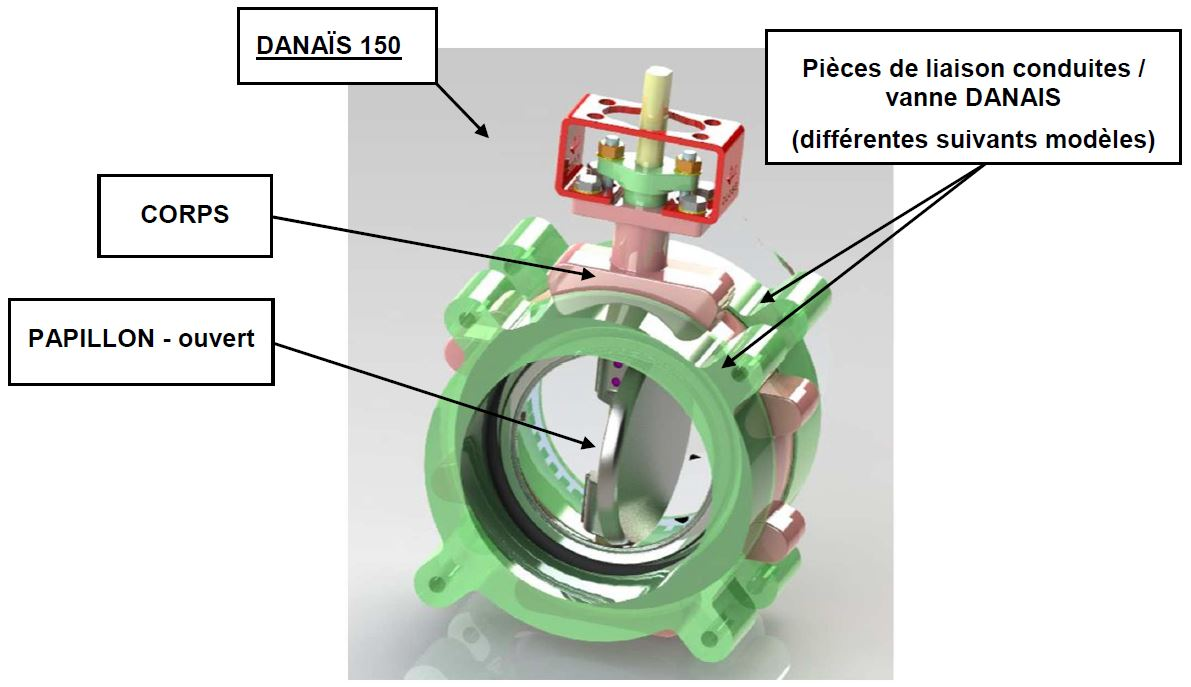
\includegraphics[width=1\textwidth]{Images/2015A.JPG} % Include the figure image
	\caption{La commande du fluide peut être manuelle, hydraulique, électrique ou pneumatique. Le fluide peut passer dans les deux sens.}
	\label{2015A} % Unique label used for referencing the figure in-text
\end{figure}

Il s'agit d'un "robinet à papillon excentré - gamme DANAÏS 150 - de la marque
AMRI de l'entreprise KSB. Le robinet, sujet de cette étude, sert à véhiculer tout type de fluides, comme des
carburants, des eaux chaudes ou brûlantes, des fluides corrosifs et/ou agressifs ou
contenant des substances solides, des huiles minérales, etc.


\begin{figure}[H] % Use [H] to suppress floating and place the figure/table exactly where it is specified in the text
	\centering % Horizontally center the figure on the page
	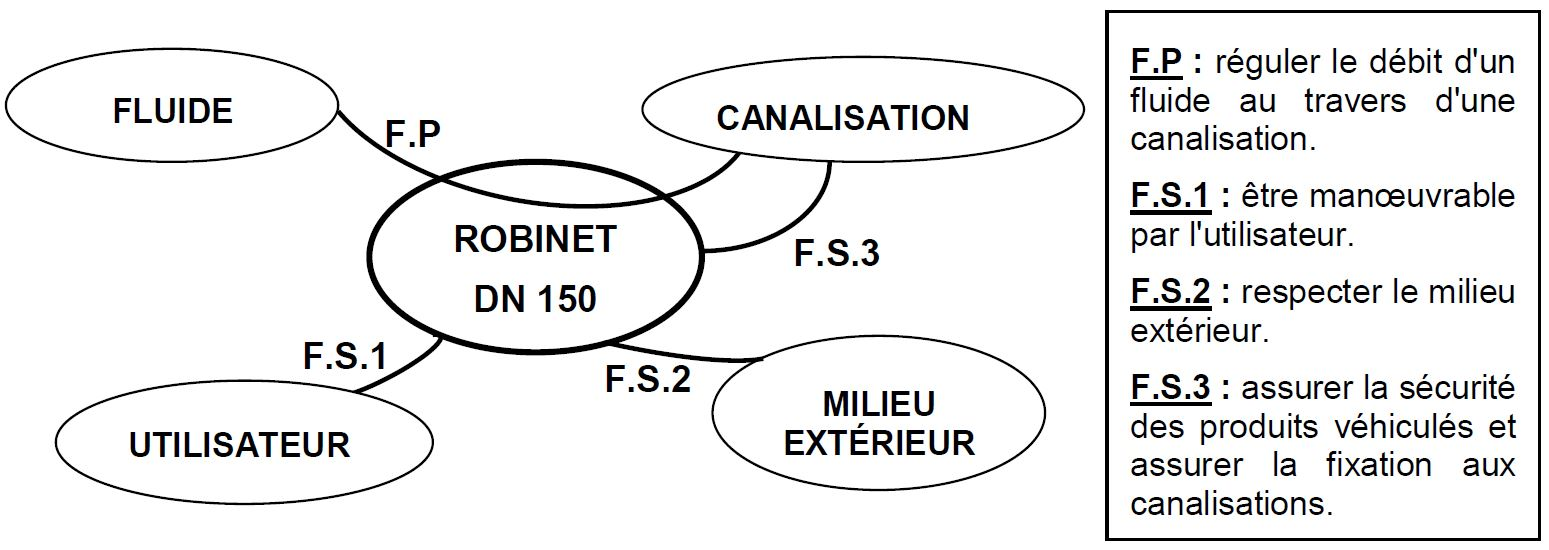
\includegraphics[width=1\textwidth]{Images/2015.JPG} % Include the figure image
	\caption{La fonction principale (F.P) du robinet est d'assurer ou d’interrompre le passage de fluides de différentes compositions (liquide - "semi-épais" - solide) et ce, à différentes températures. Pour assurer cette fonction, le mécanisme doit répondre à certaines fonctionnalités secondaires (F.S.i). Ces fonctionnalités sont classées en 3 catégories : F.S.1 - F.S.2 - F.S.3.}
	\label{2015} % Unique label used for referencing the figure in-text
\end{figure}


\begin{figure}[H] % Use [H] to suppress floating and place the figure/table exactly where it is specified in the text
	\centering % Horizontally center the figure on the page
	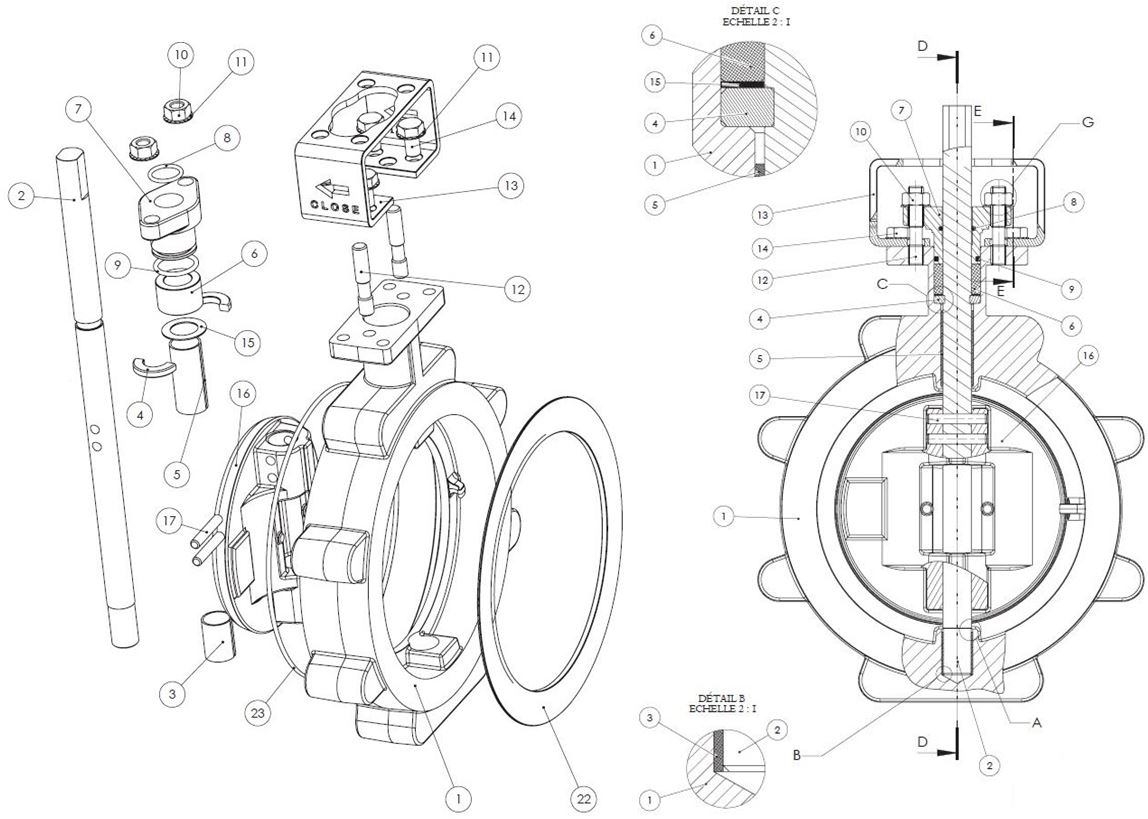
\includegraphics[width=1.1\textwidth]{Images/rob11.JPG} % Include the figure image
	\caption{La commande du fluide peut être manuelle, hydraulique, électrique ou pneumatique. Le fluide peut passer dans les deux sens.}
	\label{rob11} % Unique label used for referencing the figure in-text
\end{figure}


\begin{tcolorbox}[colback=gray!5!white,colframe=gray!75!ocre,title=Tiré du BTS 2015]\index{Exercice : Bête à corne}
\textbf{[Problème 1 : Analyse "F.P et F.S.i"]}\\


\textbf{Question 1.1 }: Pour chaque fonction "F.P et F.S.i", on demande de définir quelle est la (ou les)
\textbf{pièce(s) du robinet remplissant cette fonction} et d'associer la (ou les) \textbf{forme(s) permettant de l'assurer}. Répondre pour cela sur le tableau du document réponse DR1. Deux exemples sont proposés pour les fonctions F.S.1 et F.S.2 de façon à permettre de comprendre le principe. \\
% FP - Pièce 4 . Forme : 1/2 anneau
% FP - Pièce 13. Forme : Tôle (pliée à partir d'un parallélépipède)
% FP - Pièces 3 et 5. Forme : Tubes fendus 
% FS2 - Pièce 20. Forme : Siège plastomère (tore - anneau)
% FS2 - Pièces 6, 8, 9. Forme : Garniture Joints toriques
% FS3 - Pièce 19. Forme : Tôle sécurité " tôle cylindrique emboutie)

\end{tcolorbox}



\begin{tcolorbox}[colback=gray!5!white,colframe=gray!75!gray,title=Document réponse]
\begin{figure}[H] % Use [H] to suppress floating and place the figure/table exactly where it is specified in the text
	\centering % Horizontally center the figure on the page
	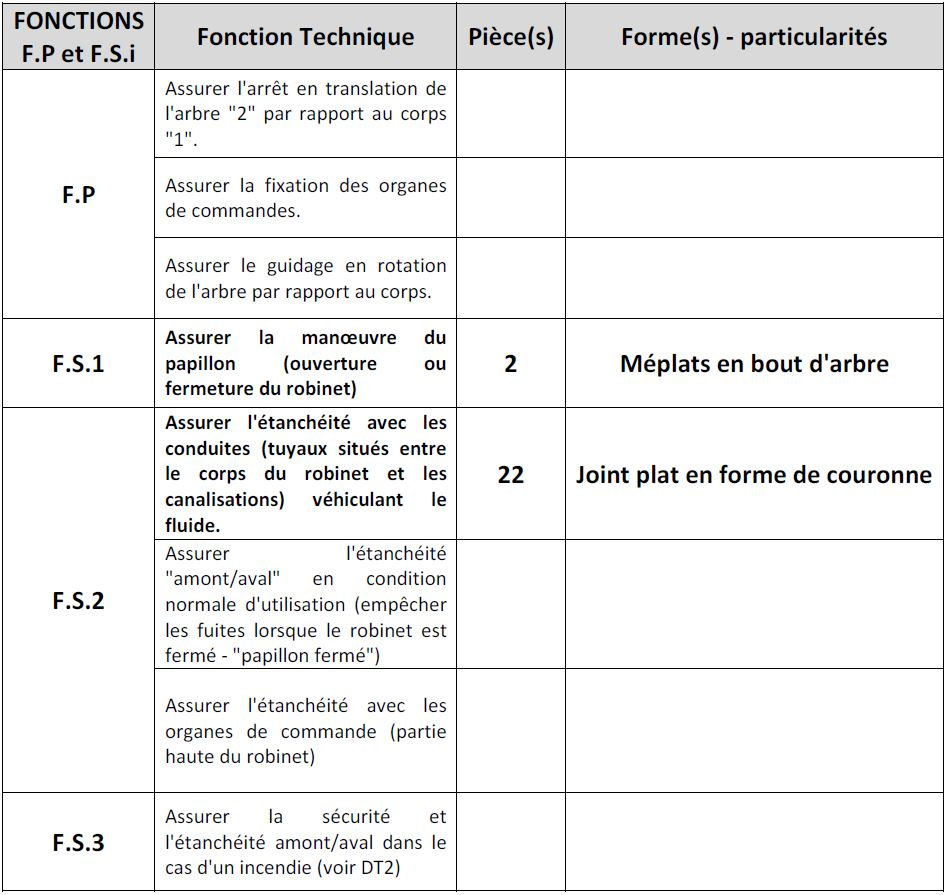
\includegraphics[width=0.9\textwidth]{Images/rob1.JPG} % Include the figure image
	\caption{Question 1.1}
	\label{rob1} % Unique label used for referencing the figure in-text
\end{figure}



\end{tcolorbox}


\section{Diagramme FAST}\index{FAST (diagramme)}

Après le diagramme bête à corne, le diagramme FAST servira davantage à entrée dans le détail du système. Le principe de la méthode de "Functional Analysis System Technique" (FAST), est de décomposer les fonctions techniques internes du produit jusqu’à établir leur relation, leur intervention, dans la réalisation des fonctions de service.\\

Elle consiste à se poser 3 questions pour chaque fonction interne du produit :
\begin{itemize}
    \item \textbf{Comment} cela est-il fait ? (accès à une fonction technique d’ordre inférieur, décomposition)
    \item \textbf{Pourquoi} cela est-il fait ? (accès à une fonction technique d’ordre supérieur, reconstruction)
    \item \textbf{Quand} cela est-il utilisé ? (recherche des simultanéités)
    
\end{itemize}



\begin{figure}[H] % Use [H] to suppress floating and place the figure/table exactly where it is specified in the text
	\centering % Horizontally center the figure on the page
	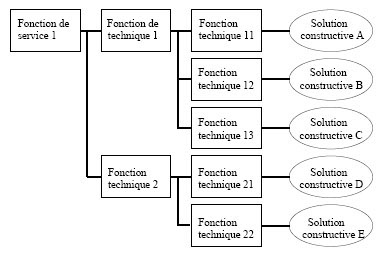
\includegraphics[width=0.8\textwidth]{Images/fast1.jpg} % Include the figure image
	\caption{Exemple type du diagramme}
	\label{fast1} % Unique label used for referencing the figure in-text
\end{figure}

Les fonctions du diagramme FAST doivent être décrites par un verbe à l'infinitif. Les réponses à chacune de ces questions ne sont ni exclusives, ni uniques. \\
Afin de permettre une compréhension aisée de tous, ce type de représentation est normé. Au niveau de la France, elle est régulée par la norme NF EN 1325-1 qui décrit les grandes lignes de cette méthode.


\subsection*{Exemple}
Il est possible de représenter l'une des fonctions de service d'un pilote automatique de bateau. Le but sera, par exemple : «\textbf{ Maintenir le cap} ». Le diagramme FAST pourra être construit de la manière suivante :

\begin{figure}[H] % Use [H] to suppress floating and place the figure/table exactly where it is specified in the text
	\centering % Horizontally center the figure on the page
	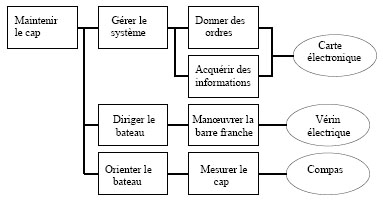
\includegraphics[width=0.8\textwidth]{Images/fast2.jpg} % Include the figure image
	\caption{Fonction "Maintenir le cap" pour un bateau}
	\label{fast2} % Unique label used for referencing the figure in-text
\end{figure}


\section{Diagramme SADT}\index{SADT (diagramme)}
SADT (en anglais structured analysis and design technique), connue aussi sous le label IDEF0 (en anglais Integration Definition for Function Modeling). Elle se répandit vers la fin des années 1980 comme l'un des standards de description graphique d'un système complexe par analyse fonctionnelle descendante, c'est-à-dire que l'analyse chemine du général (dit « niveau A-0 ») vers le particulier et le détaillé (dits « niveaux $A_{ijk}$ »). SADT est une démarche systémique de modélisation d'un système complexe ou d'un processus opératoire.

\begin{figure}[H] % Use [H] to suppress floating and place the figure/table exactly where it is specified in the text
	\centering % Horizontally center the figure on the page
	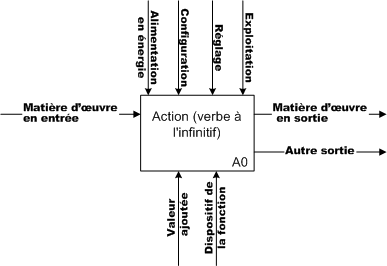
\includegraphics[width=0.7\textwidth]{Images/Sadt.png} % Include the figure image
	\caption{Représentation théorique d'une fonction.}
	\label{sadt} % Unique label used for referencing the figure in-text
\end{figure}
Une représentation de la fonction USINER pourrait être la suivante :
\begin{figure}[H] % Use [H] to suppress floating and place the figure/table exactly where it is specified in the text
	\centering % Horizontally center the figure on the page
	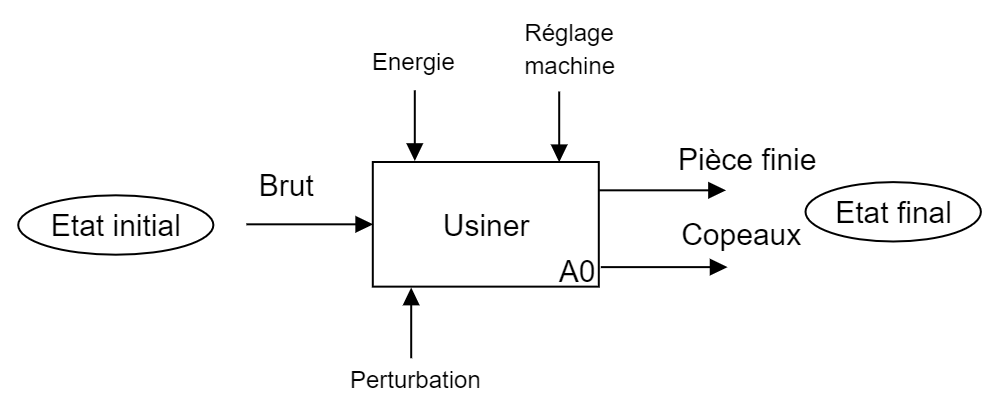
\includegraphics[width=1\textwidth]{Images/sadt1.png} % Include the figure image
	\caption{Boite principale (A0) de la fonction : Usiner une pièce.}
	\label{sadt1} % Unique label used for referencing the figure in-text
\end{figure}

\subsection*{Exemple : Sécateur automatique}

\begin{figure}[H]
\fbox{
    \begin{minipage}[c]{.46\linewidth}
        \centering
        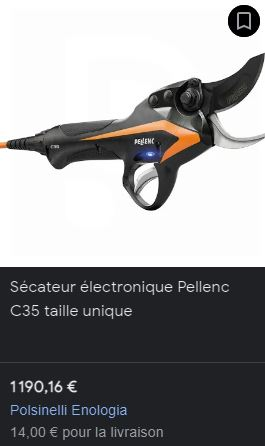
\includegraphics[width=0.6\textwidth]{Images/seca3.JPG}
        \caption{Système Sécateur}
    \end{minipage}
}
    \hfill%
    \begin{minipage}[c]{.46\linewidth}
        \centering
        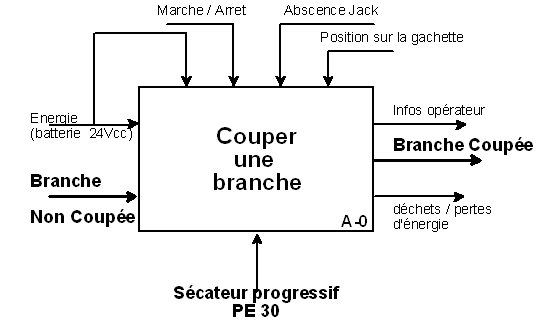
\includegraphics[width=1.2\textwidth]{Images/seca1.png}
        \caption{Boite principale de la fonction A-0}
    \end{minipage}

\end{figure}

Toujours dans les débuts des sujets de BTS, vous devrez comprendre le système dans son ensemble et répondre sur la validation d'exigences du cahier des charges. Ici, une question possible serait :\\
\textbf{Question} : A l'aide de la représentation SADT ci-dessous, comment le sécateur commande la vitesse avec laquelle la lame se ferme pour couper une branche ?



\begin{figure}[H] % Use [H] to suppress floating and place the figure/table exactly where it is specified in the text
	\centering % Horizontally center the figure on the page
	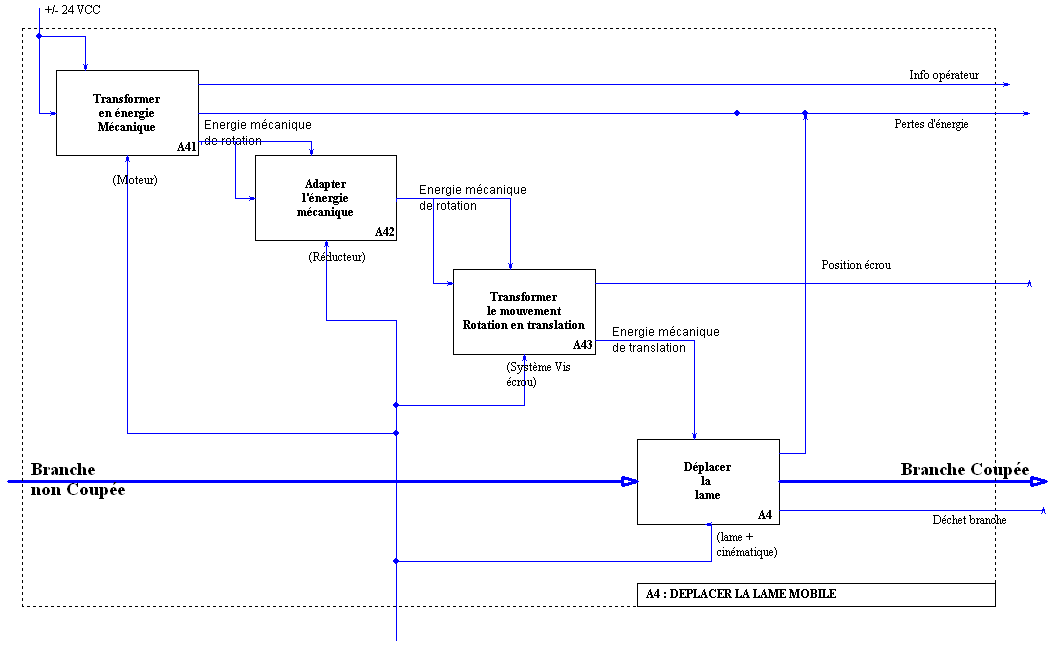
\includegraphics[width=1.1\textwidth]{Images/seca2.png} % Include the figure image
	\caption{Représentation théorique d'une fonction.}
	\label{seca2} % Unique label used for referencing the figure in-text
\end{figure}


\section{Chaîne fonctionnelle}
C'est une représentation que vous observerez sûrement moins que les autres car elle décrit un système dans son ensemble. En générale, nous nous intéresserons à une pièce d'un système,  son industrialisation, sa fabrication, son contrôle ; et c'est déjà beaucoup ! Mais vous pourrez croiser cette schématisation dans certains sujets pour avoir une idée du rôle de la pièce dans le système global.

\begin{figure}[H] % Use [H] to suppress floating and place the figure/table exactly where it is specified in the text
	\centering % Horizontally center the figure on the page
	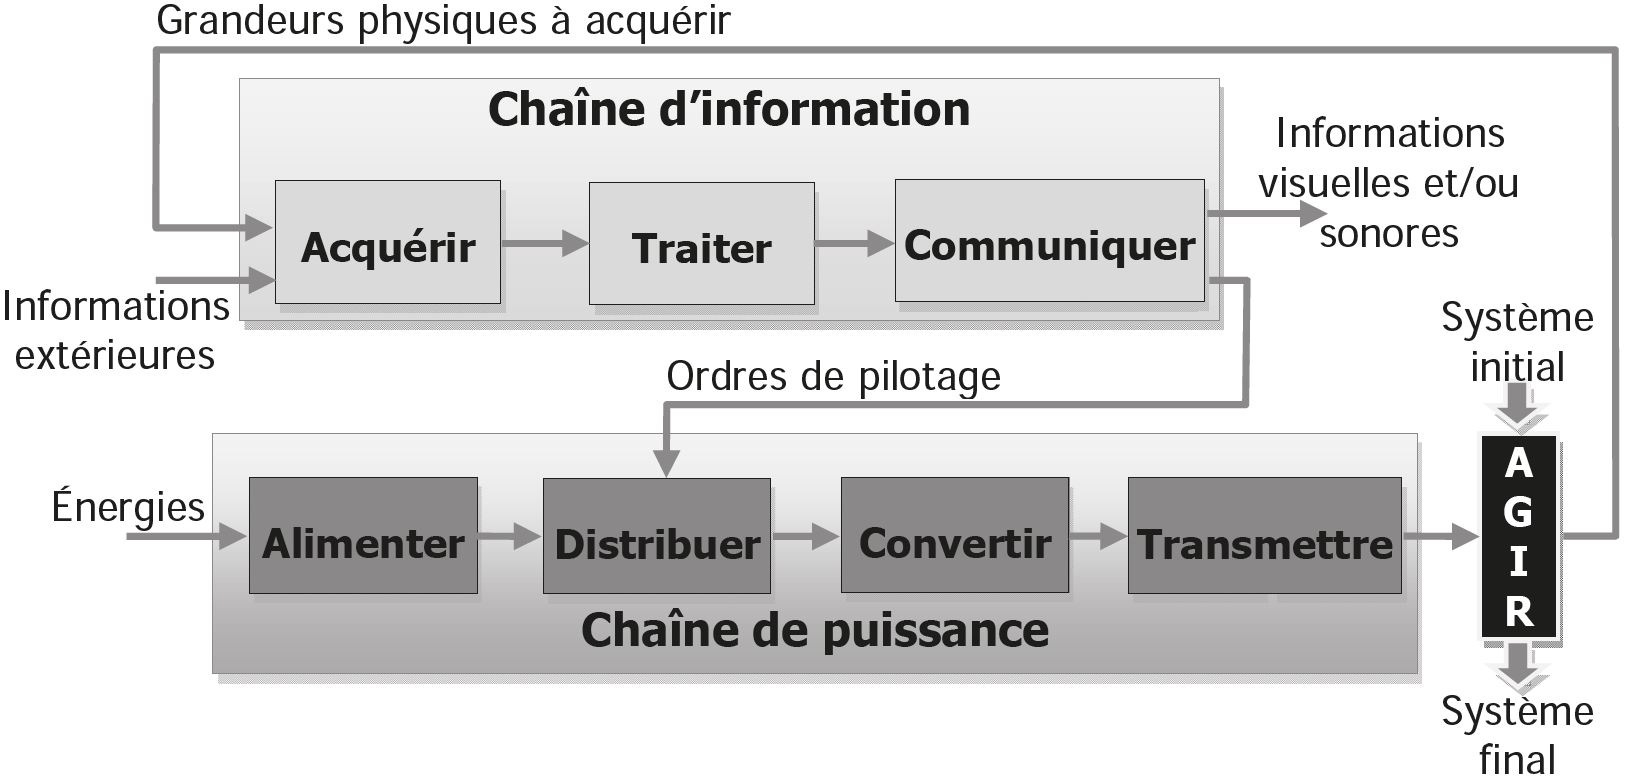
\includegraphics[width=1.1\textwidth]{Images/chaine1.JPG} % Include the figure image
	\caption{Représentation d'une chaîne fonctionnelle complète.}
	\label{chaine1} % Unique label used for referencing the figure in-text
\end{figure}

Une chaîne fonctionnelle est une combinaison d'une chaînes d’information et d'une chaîne de puissance. On peut aussi remplacer le nom « chaîne de puissance » par « chaîne d’énergie » car l’énergie correspond à la puissance consommée par le système pendant un certain temps.

\subsection{Chaîne d'information}
Pour les deux chaînes, chaque bloc (Acquérir, Distribuer etc.) fonctionne grâce à des éléments prévus pour effectuer la fonction du bloc. Le bloc \textbf{acquérir} ne contiendra que des éléments pour acquérir une \textbf{information} (car on est dans la chaîne d'information). Par exemple, un \textbf{capteur} peut acquérir une information.
\begin{figure}[H] % Use [H] to suppress floating and place the figure/table exactly where it is specified in the text
	\centering % Horizontally center the figure on the page
	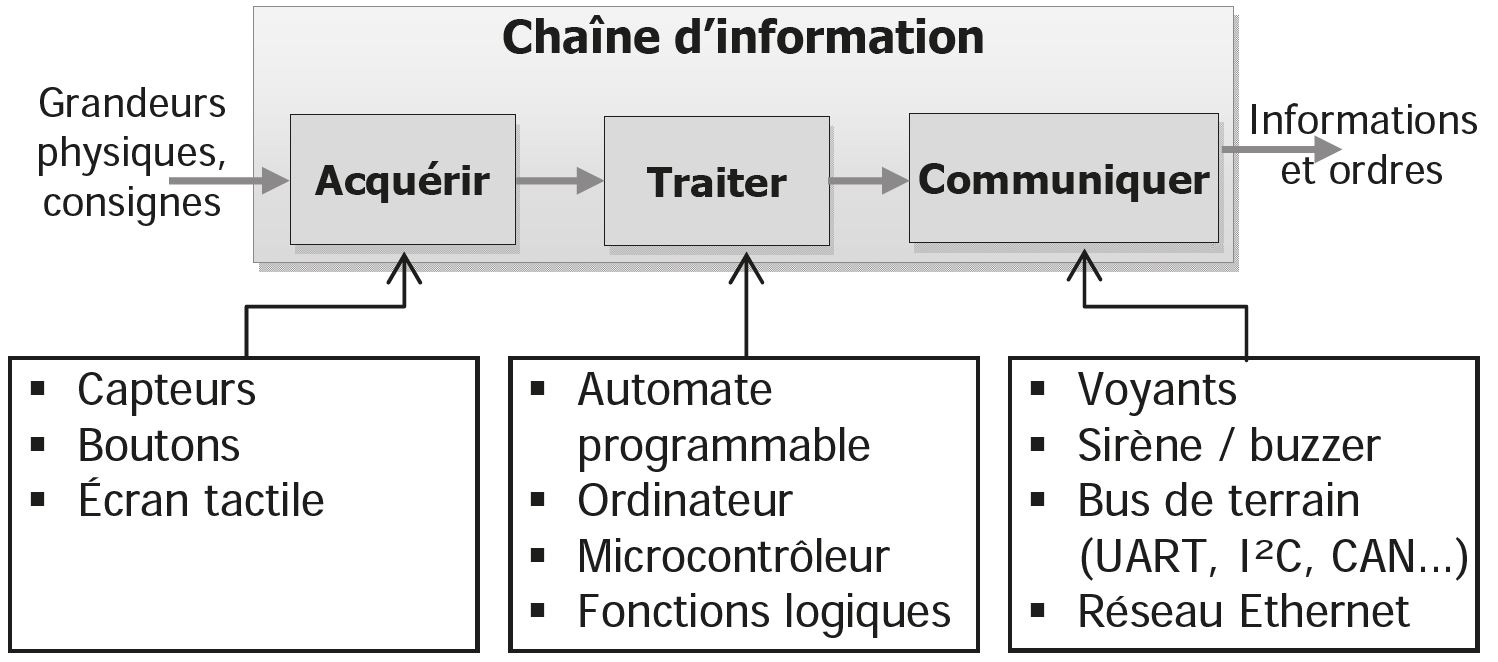
\includegraphics[width=1\textwidth]{Images/chaine2.JPG} % Include the figure image
	\caption{Représentation d'une chaîne d'information et des éléments pouvant constituer les différents blocs.}
	\label{chaine2} % Unique label used for referencing the figure in-text
\end{figure}


\subsection{Chaîne d'énergie (ou de puissance)}
Ici, dans le bloc transmettre, on pourrait aussi retrouver les courroies de transmission, les engrenages ou encore les systèmes roues-vis sans fin.
\begin{figure}[H] % Use [H] to suppress floating and place the figure/table exactly where it is specified in the text
	\centering % Horizontally center the figure on the page
	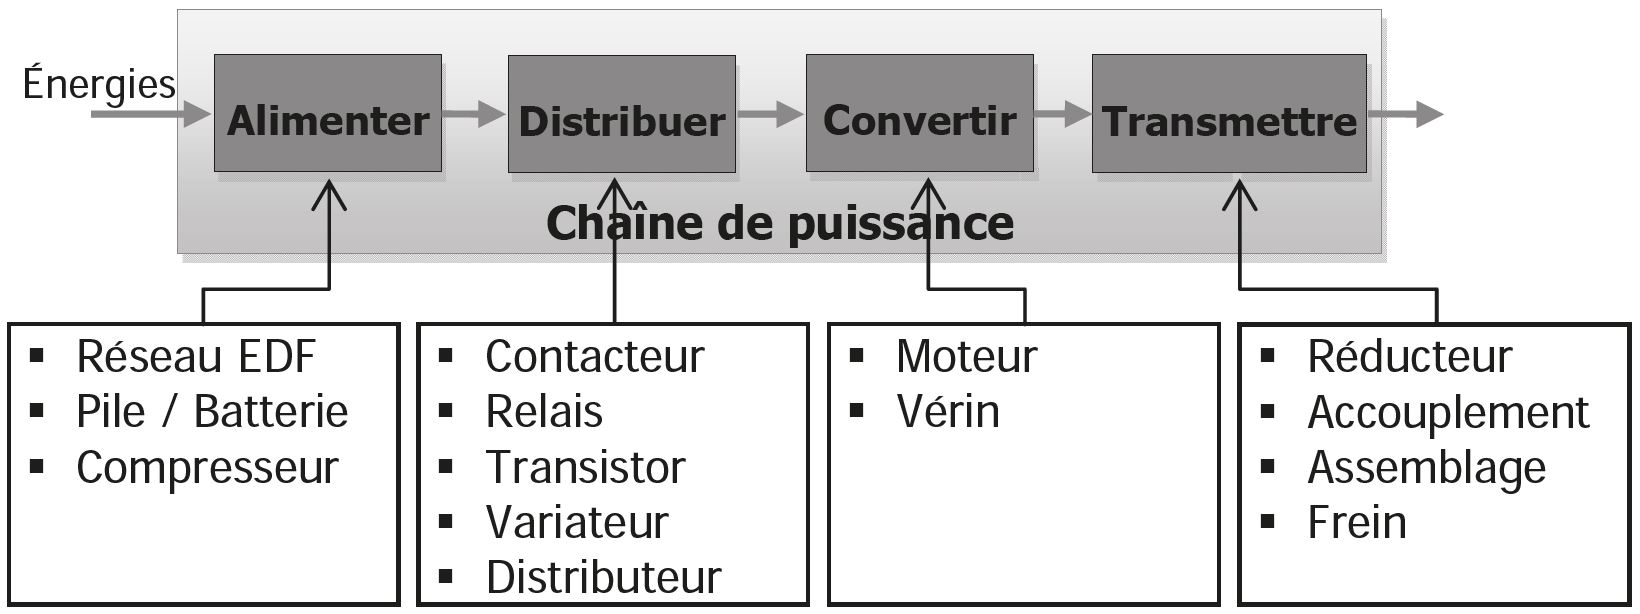
\includegraphics[width=1\textwidth]{Images/chaine3.JPG} % Include the figure image
	\caption{Représentation d'une chaîne de puissance et des éléments pouvant constituer les différents blocs.}
	\label{chaine3} % Unique label used for referencing the figure in-text
\end{figure}

\subsection*{Exemple}
Dans une centrale hydroélectrique, on peut représenter un système qui pilote l’orientation des pales d'une turbine suivant le niveau de la rivière. Si les pâles ont un angle faible, le débit en sortie sera plus faible que pour un angle plus grand.
\begin{figure}[H] % Use [H] to suppress floating and place the figure/table exactly where it is specified in the text
	\centering % Horizontally center the figure on the page
	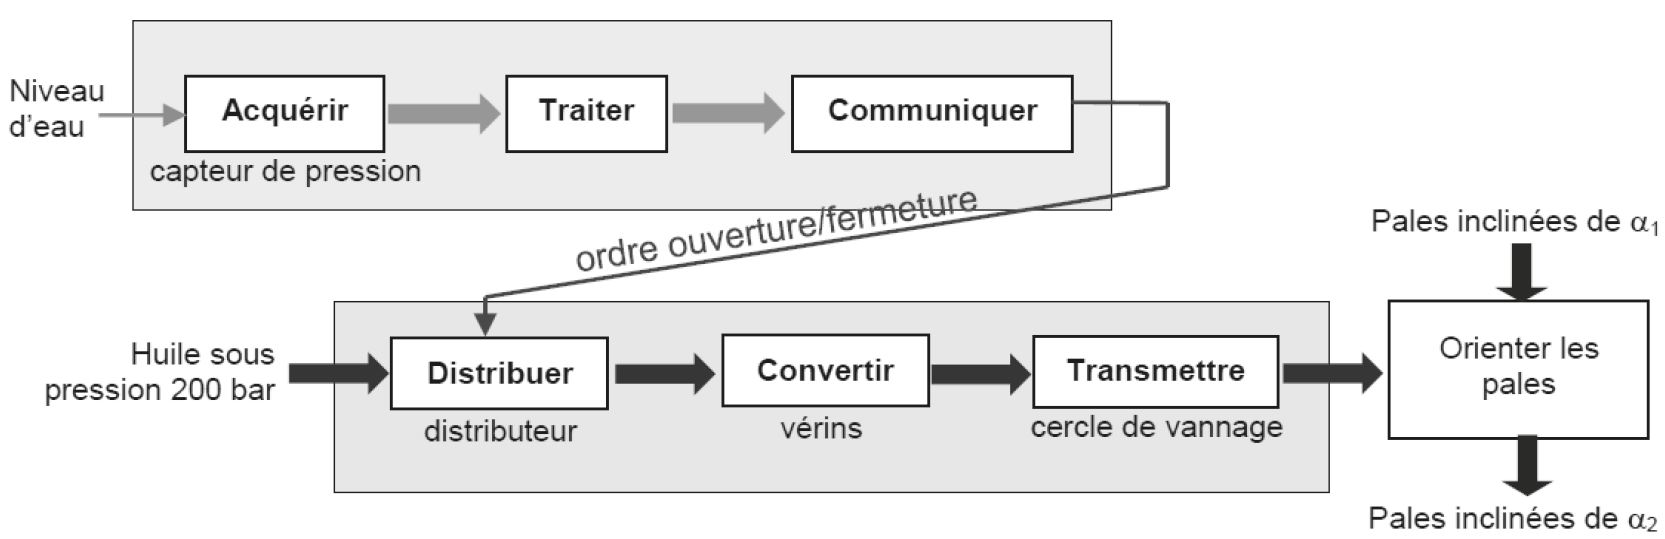
\includegraphics[width=1\textwidth]{Images/chaine4.JPG} % Include the figure image
	\caption{Chaîne fonctionnelle du système d'orientation des pâles d'une centrale hydroélectrique.}
	\label{chaine4} % Unique label used for referencing the figure in-text
\end{figure}

\subsection{Exercice}
À partir des documents techniques fournis, compléter les chaînes d’information et d’énergie en donnant les solutions techniques et les grandeurs « effort » et « flux » correspondant à la puissance transmise jusqu’au niveau de la
chaîne d’entraînement.

\begin{tcolorbox}[colback=gray!5!white,colframe=gray!75!ocre,title=Fenêtre de toit VELUX]\index{Exercice : Fenêtre de toit VELUX}

\begin{figure}[H] % Use [H] to suppress floating and place the figure/table exactly where it is specified in the text
	\centering % Horizontally center the figure on the page
	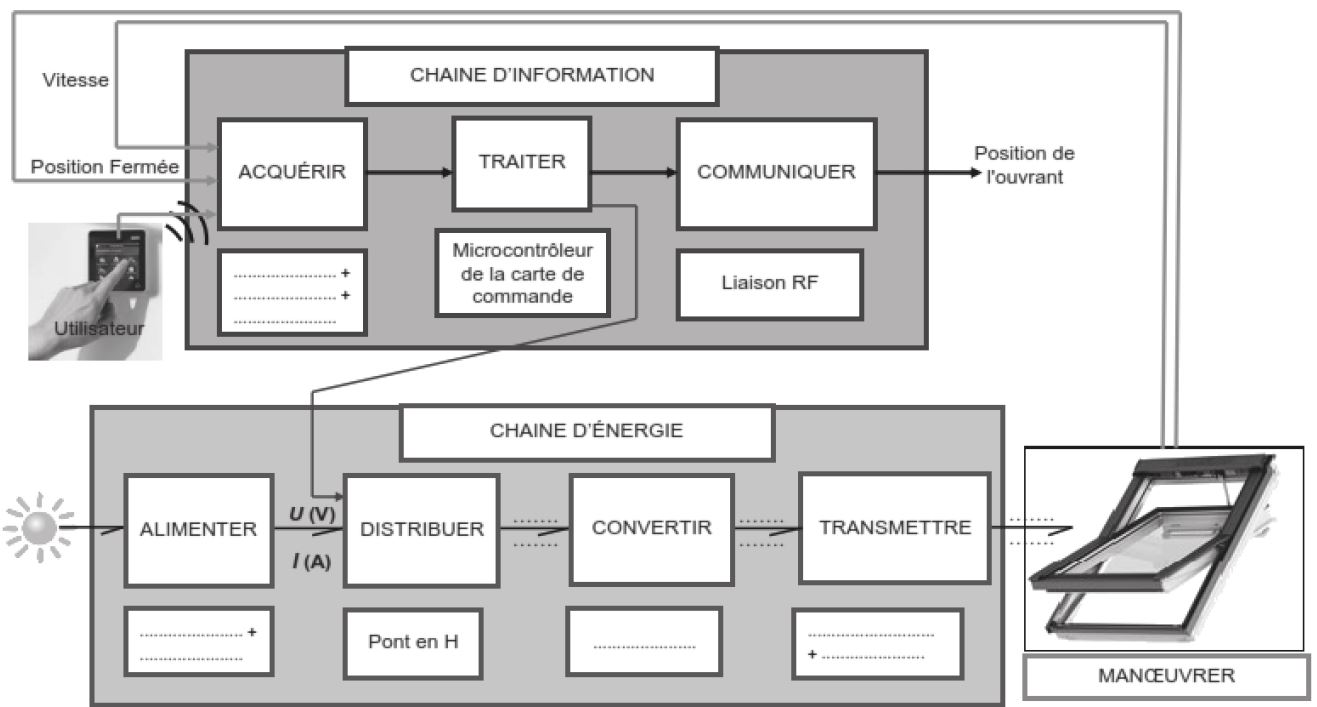
\includegraphics[width=1\textwidth]{Images/chaine5.JPG} % Include the figure image
	\caption{Complétez la chaîne fonctionnelle à l'aide du document réponse}
	\label{chaine5} % Unique label used for referencing the figure in-text
\end{figure}
\end{tcolorbox}


\begin{tcolorbox}[colback=gray!5!white,colframe=gray!75!gray,title=Document réponse]
\begin{figure}[H] % Use [H] to suppress floating and place the figure/table exactly where it is specified in the text
	\centering % Horizontally center the figure on the page
	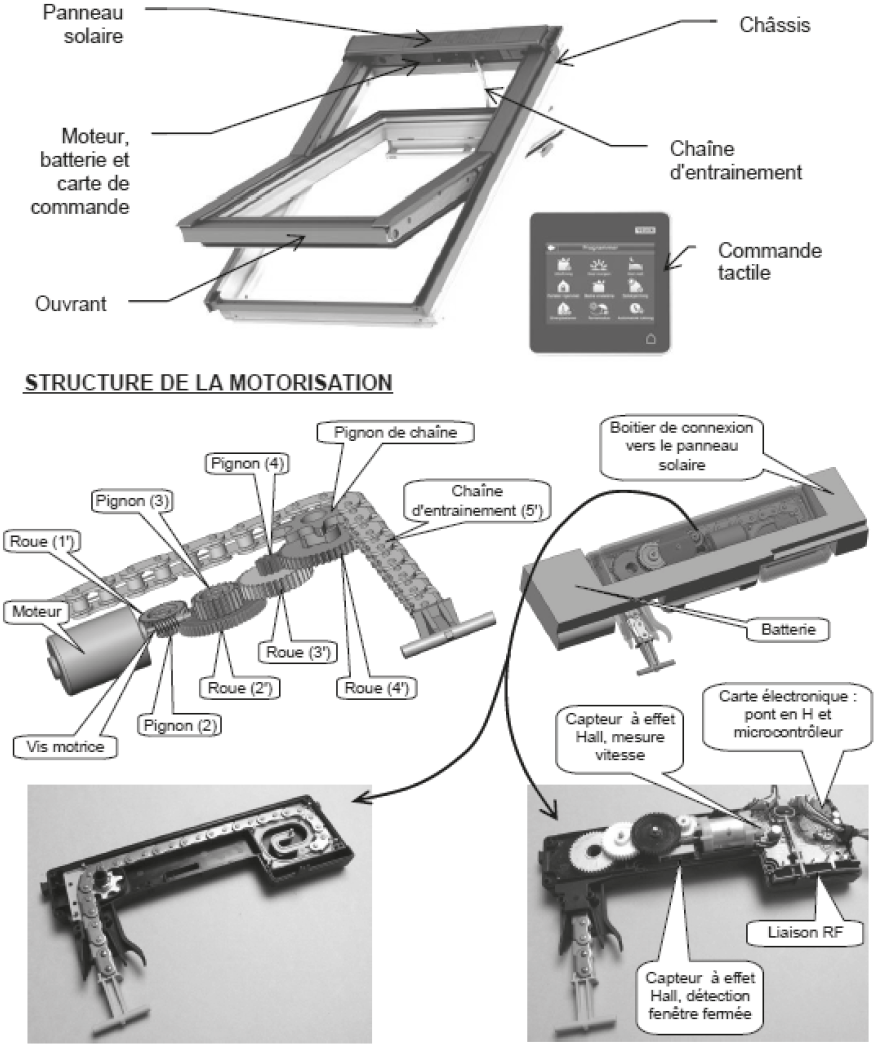
\includegraphics[width=1\textwidth]{Images/chaine6.png} % Include the figure image
	\caption{Question 1.1}
	\label{chaine6} % Unique label used for referencing the figure in-text
\end{figure}
\end{tcolorbox}







%----------------------------------------------------------------------------------------
%	PRESENTING INFORMATION/RESULTS EXAMPLES CHAPTER
%----------------------------------------------------------------------------------------

\chapterimage{Images/A6.jpg} % Chapter heading image
\chapterspaceabove{6.25cm} % Whitespace from the top of the page to the chapter title on chapter pages
\chapterspacebelow{7.5cm} % Amount of vertical whitespace from the top margin to the start of the text on chapter pages

%------------------------------------------------

\chapter{Dessine-moi une pièce}

\section{Dessin de définition. A venir}\index{Table}
%[Cours 1.2]
%3. Dessin de définition, vues, coupes, trous etc
%4. Cote intrinsèque, intro specif GPS [comment prouver que deux plans sont parallèles à un intervalle de tolérances près? %"Dire ce que l'on veut - deux plans // et aussi dire comment on mesure s'ils le sont, ou si la pièce est mauvaise] , état %de surface



%----------------------------------------------------------------------------------------
%	PRESENTING INFORMATION/RESULTS EXAMPLES CHAPTER
%----------------------------------------------------------------------------------------

\chapterimage{Images/AA12.jpg} % Chapter heading image
\chapterspaceabove{6.25cm} % Whitespace from the top of the page to the chapter title on chapter pages
\chapterspacebelow{7.5cm} % Amount of vertical whitespace from the top margin to the start of the text on chapter pages

%------------------------------------------------

\chapter{Spécification géométrique des produits}
\section{A venir}




%----------------------------------------------------------------------------------------
%	PRESENTING INFORMATION/RESULTS EXAMPLES CHAPTER
%----------------------------------------------------------------------------------------

\chapterimage{Images/A6.jpg} % Chapter heading image
\chapterspaceabove{6.25cm} % Whitespace from the top of the page to the chapter title on chapter pages
\chapterspacebelow{7.5cm} % Amount of vertical whitespace from the top margin to the start of the text on chapter pages

%------------------------------------------------


	




\newpage
\section{ANNEXE}


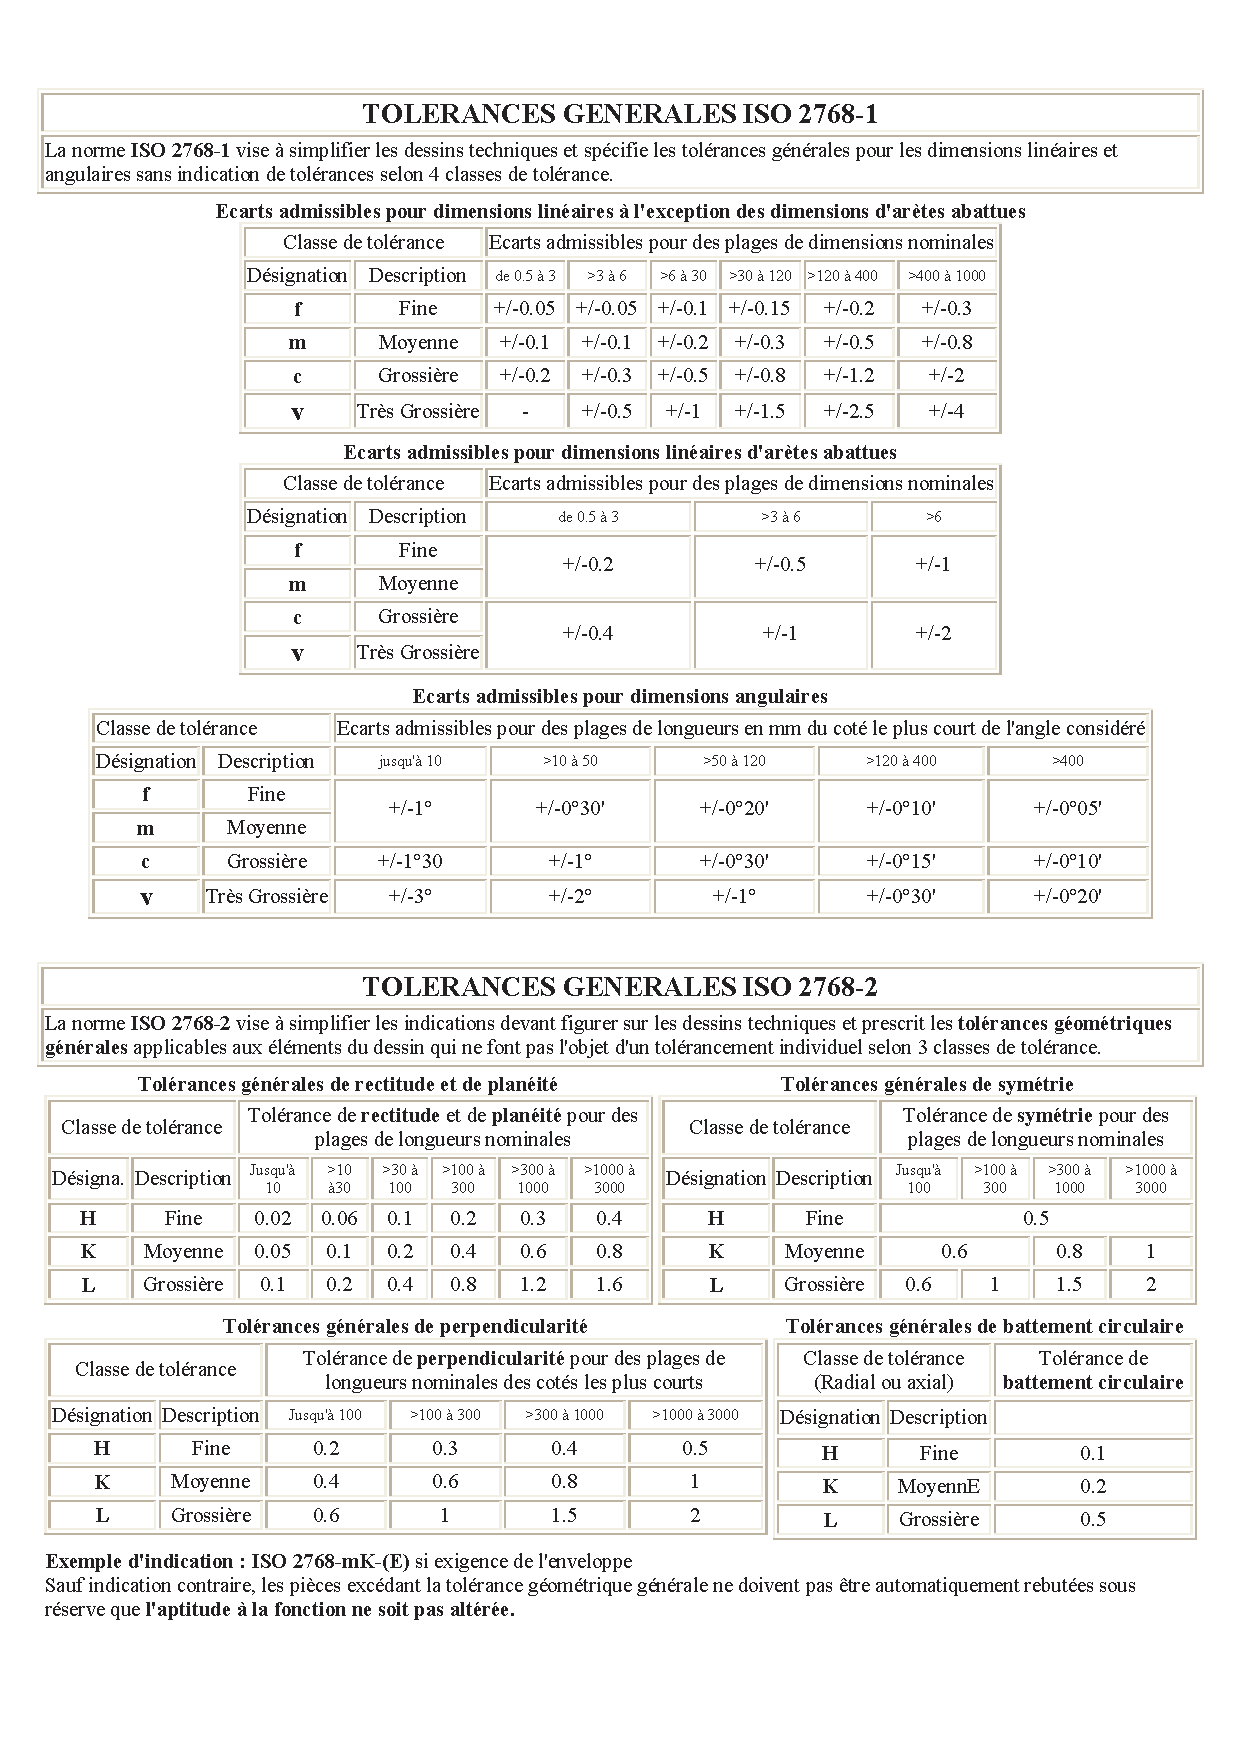
\includepdf{Tolerance-generale-ISO-2768.pdf}\index{ISO 2768-1}

\phantomsection
\addcontentsline{toc}{chapter}{\textcolor{ocre}{Index}} % Add an Index heading to the table of contents
\printindex % Output the index


\end{document}


